\documentclass{beamer}

\usepackage[beamer]{shortcut}
\usepackage{bibentry}

\graphicspath{{./images/}}
\usepackage[square]{natbib}


\definecolor{tomcolor}{rgb}{0.,.3,.6}
\definecolor{kw}{RGB}{0,112,26}
\definecolor{var}{RGB}{0,133,182}
\definecolor{func}{RGB}{0,35,126}
\definecolor{palegreen}{RGB}{236,240,241}
\setbeamercolor{bgcolor}{fg=black!60,bg=palegreen}

\usepackage[procnames]{listings}
\lstset{%
language   = Python,%
% basicstyle = \ttfamily\setstretch{1},%
linewidth= \linewidth,
numberstyle=\tiny,
stepnumber=1,
numbersep=8pt, %
frame=shadowbox,
rulesepcolor=\color{black},
procnamekeys={def,class},
procnamestyle=\color{oneblue}\textbf,
literate={*}{{\char42}}1
         {-}{{\char45}}1
         {\ }{{\copyablespace}}1
}

\lstset{basicstyle=\color{tomcolor}\scriptsize\ttfamily}

\setbeamercovered{invisible}



\newcommand{\rem}{\underline{Rem}:~}


\def\keypoint#1{\hspace{0pt plus 1 filll}\textcolor{gray}{#1}}
\def\mycite#1{\keypoint{\small\citep{#1}}}
\def\tT{\widetilde{T}}
\def\myitem{\hskip1ex{\color{linkcolor} $\blacktriangleright$}\hskip.3em}

\institute{\\ INRIA Saclay - MIND Team}
\author{Thomas Moreau}
\title{
	Modeling Brain Waveforms with Convolutional Dictionary Learning and Point Processes
}

\setbeamertemplate{title page}[frame]
\def\extraLogo{}
\collaborators{
    Tom Dupré La Tour, Mainak Jas, Alexandre Gramfort,\\
    Cédric Allain, Lindsey Power, Tim Bardouille
}

\begin{document}

\begin{frame}
	\titlepage
    \nobibliography{library.bib}
\end{frame}



\frame{
    \frametitle{Context: functional Neuroimaging}

    \large {\bf Goal:}
    Study the brain mechanisms while it is functioning.\\[3em]

    {\bf Outputs:}\\[1em]
    \begin{itemize}\itemsep1em
        \item {\bf Functional Atlases:} Link areas of the brain to specific cognitive functions.
        \item {\bf Functional Connectivity:} Highlight the information flow in the brain.
        \item {\bf Healthcare:} Develop bio-markers for neurological disorders.
    \end{itemize}
}

\frame[t]{
    \frametitle{Context: functional Neuroimaging}

    {\large How to record living brains electrical activity: \textbf{Electrophysiology}}\\[.3em]

    \centering\large Direct measurement: intracranial EEG.\\[.5em]
        \centering
        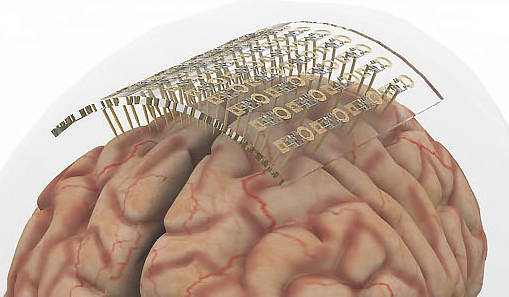
\includegraphics[width=.7\textwidth]{brain_probe.jpg}\\[1em]
        \begin{columns}
            \techterm{\color{darkblue} High Localization}%
            \techterm{Low Resolution}%
            \techterm{Invasive}%
        \end{columns}
}


\frame[t]{
    \frametitle{Context: functional Neuroimaging}

    {\large How to record living brains electrical activity: \textbf{Electrophysiology}}\\[.3em]

    \large\centering Remote measurement: M/EEG.\\[-.5em]
    \begin{columns}[T]
        \column{.35\textwidth}
        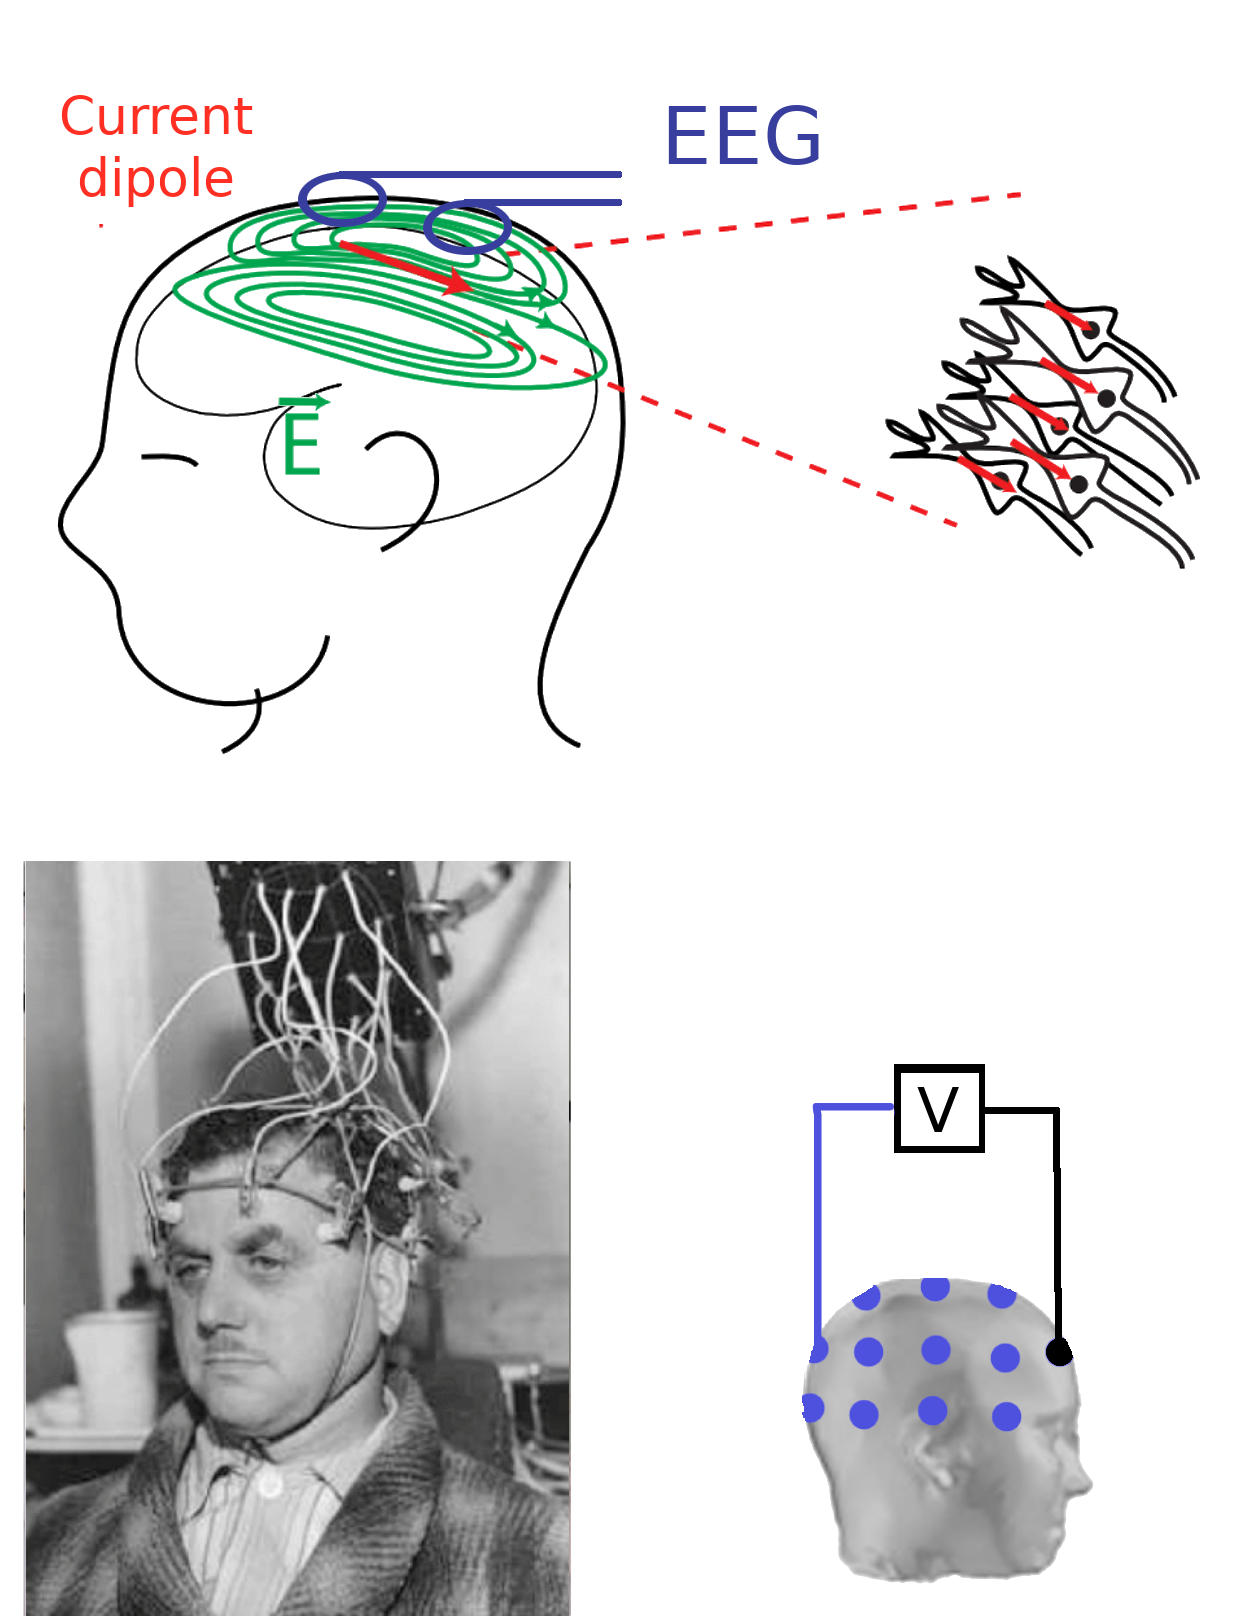
\includegraphics[width=\textwidth]{eeg_presentation}
        \column{.35\textwidth}
        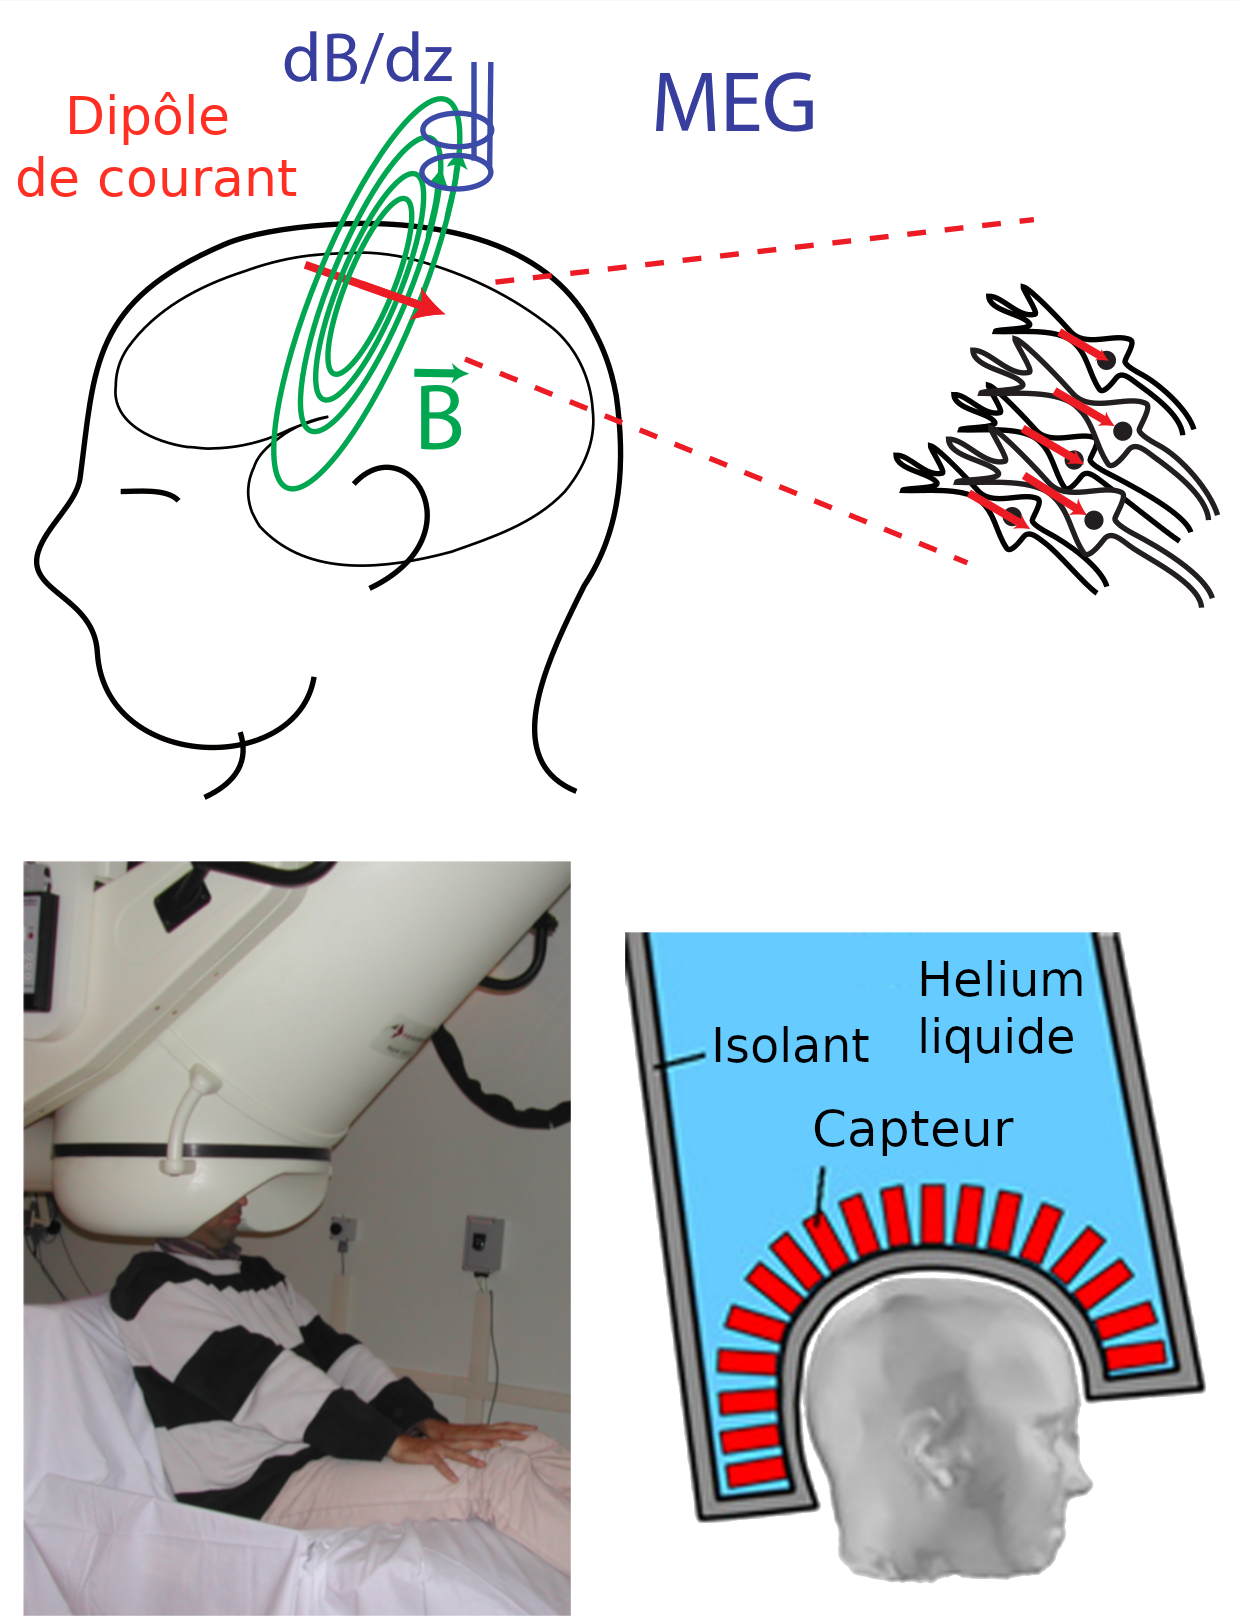
\includegraphics[width=\textwidth]{meg_presentation}
    \end{columns}
    % \only<2>{
    \begin{columns}
        \techterm{No Localization}%
        \techterm{\color{darkblue} Global}%
        \techterm{\color{darkblue} Non Invasive}%
    \end{columns}
    % }

}

\frame{
    \frametitle{M/EEG signals}

    {\Large\bf Multivariate time-series $X$}\\[1em]

    \centering
    \alt<3>{
        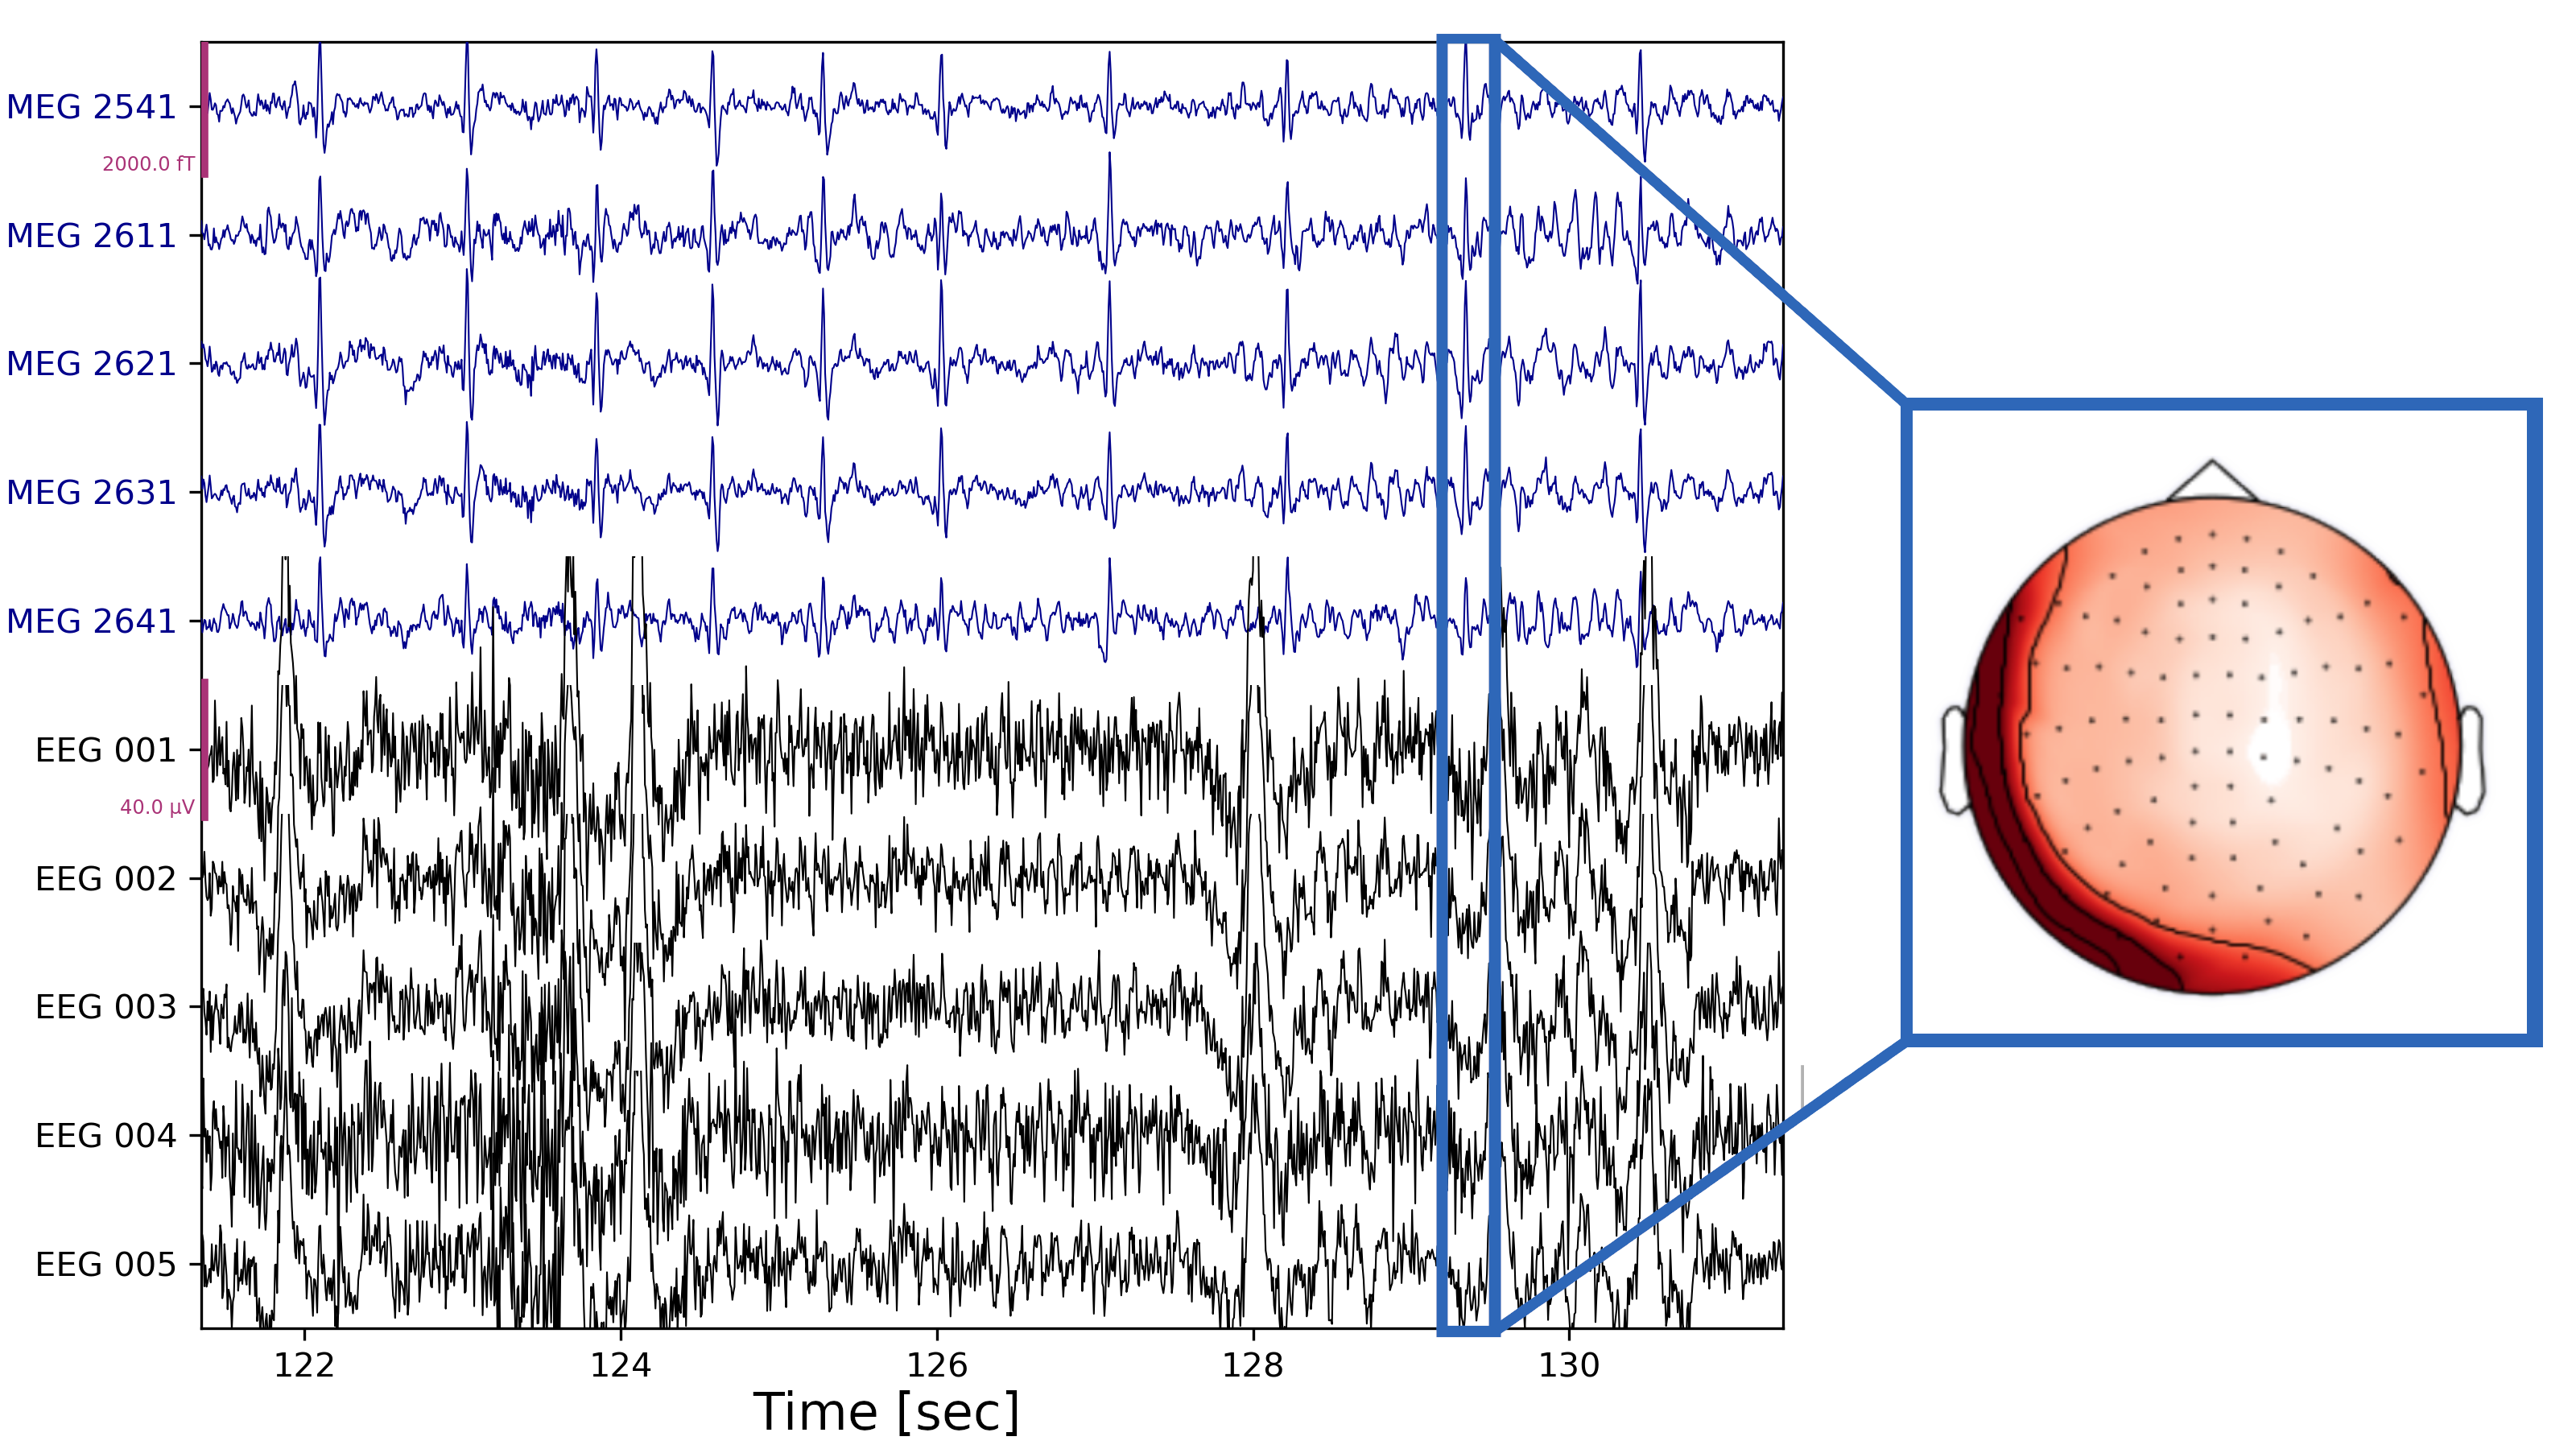
\includegraphics[width=.9\textwidth]{meeg_data_highlight}
    }{
        \alt<1>{
            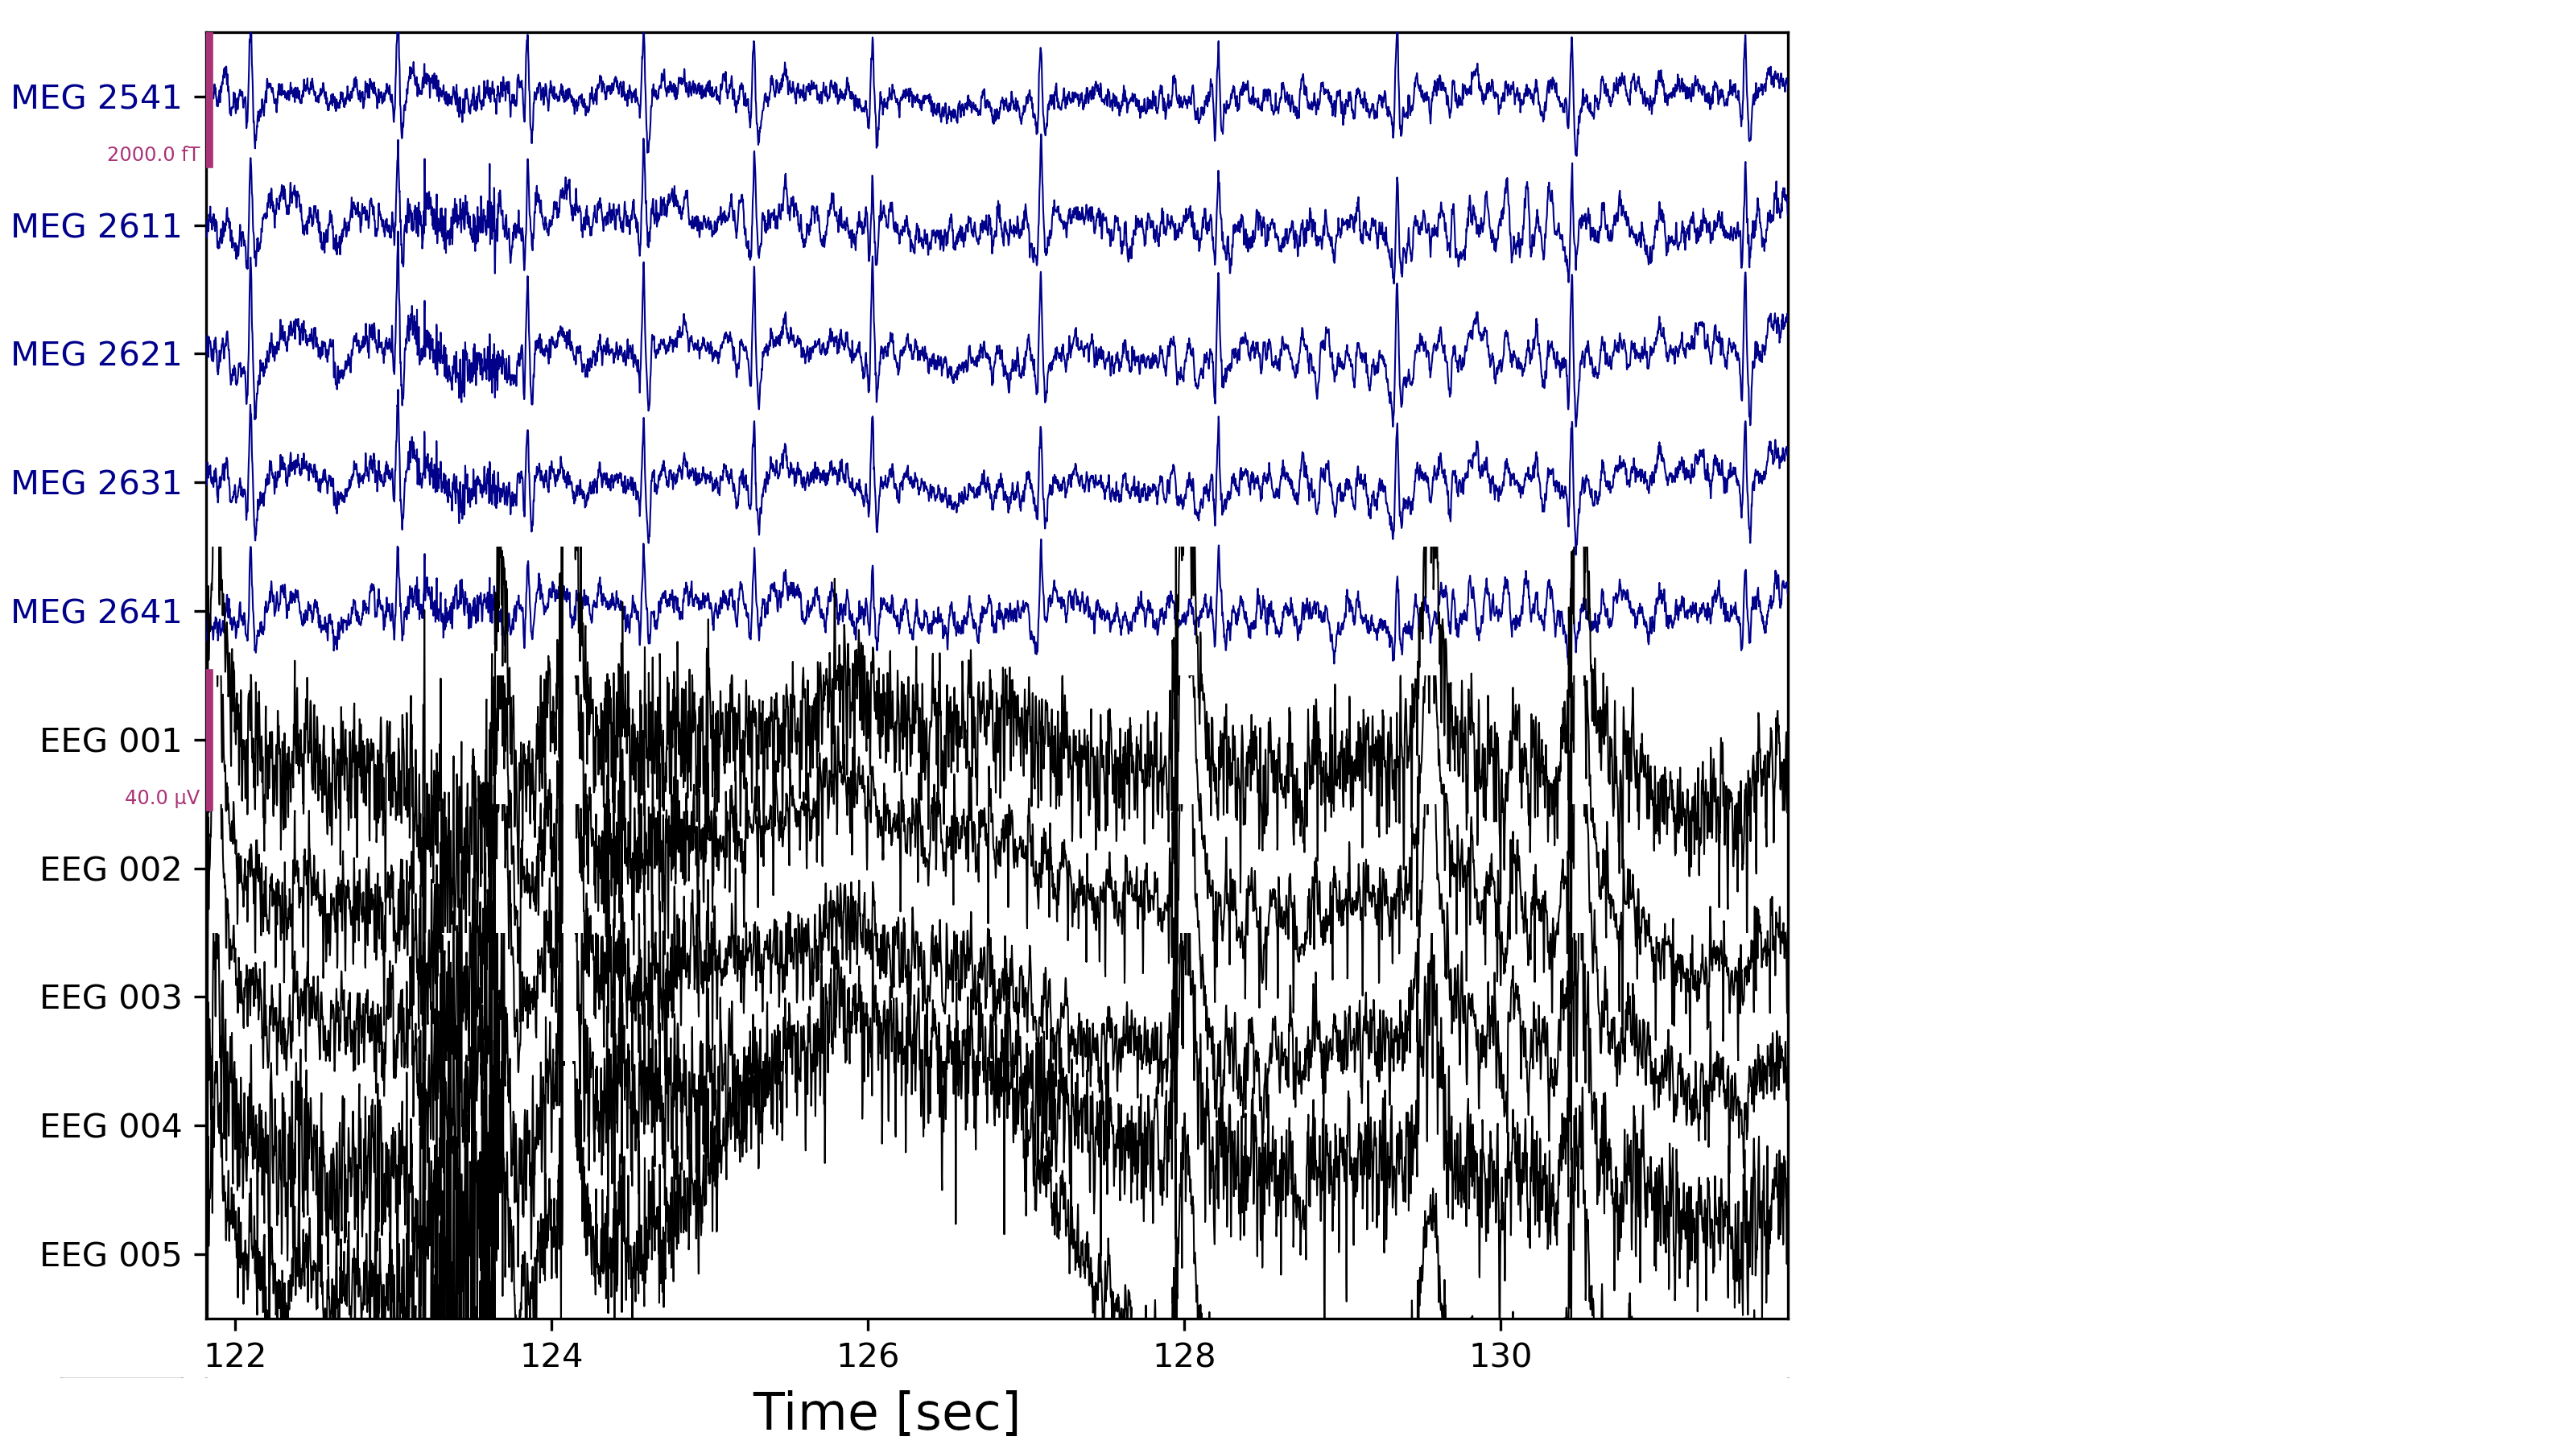
\includegraphics[width=.9\textwidth]{meeg_data}
        }{
            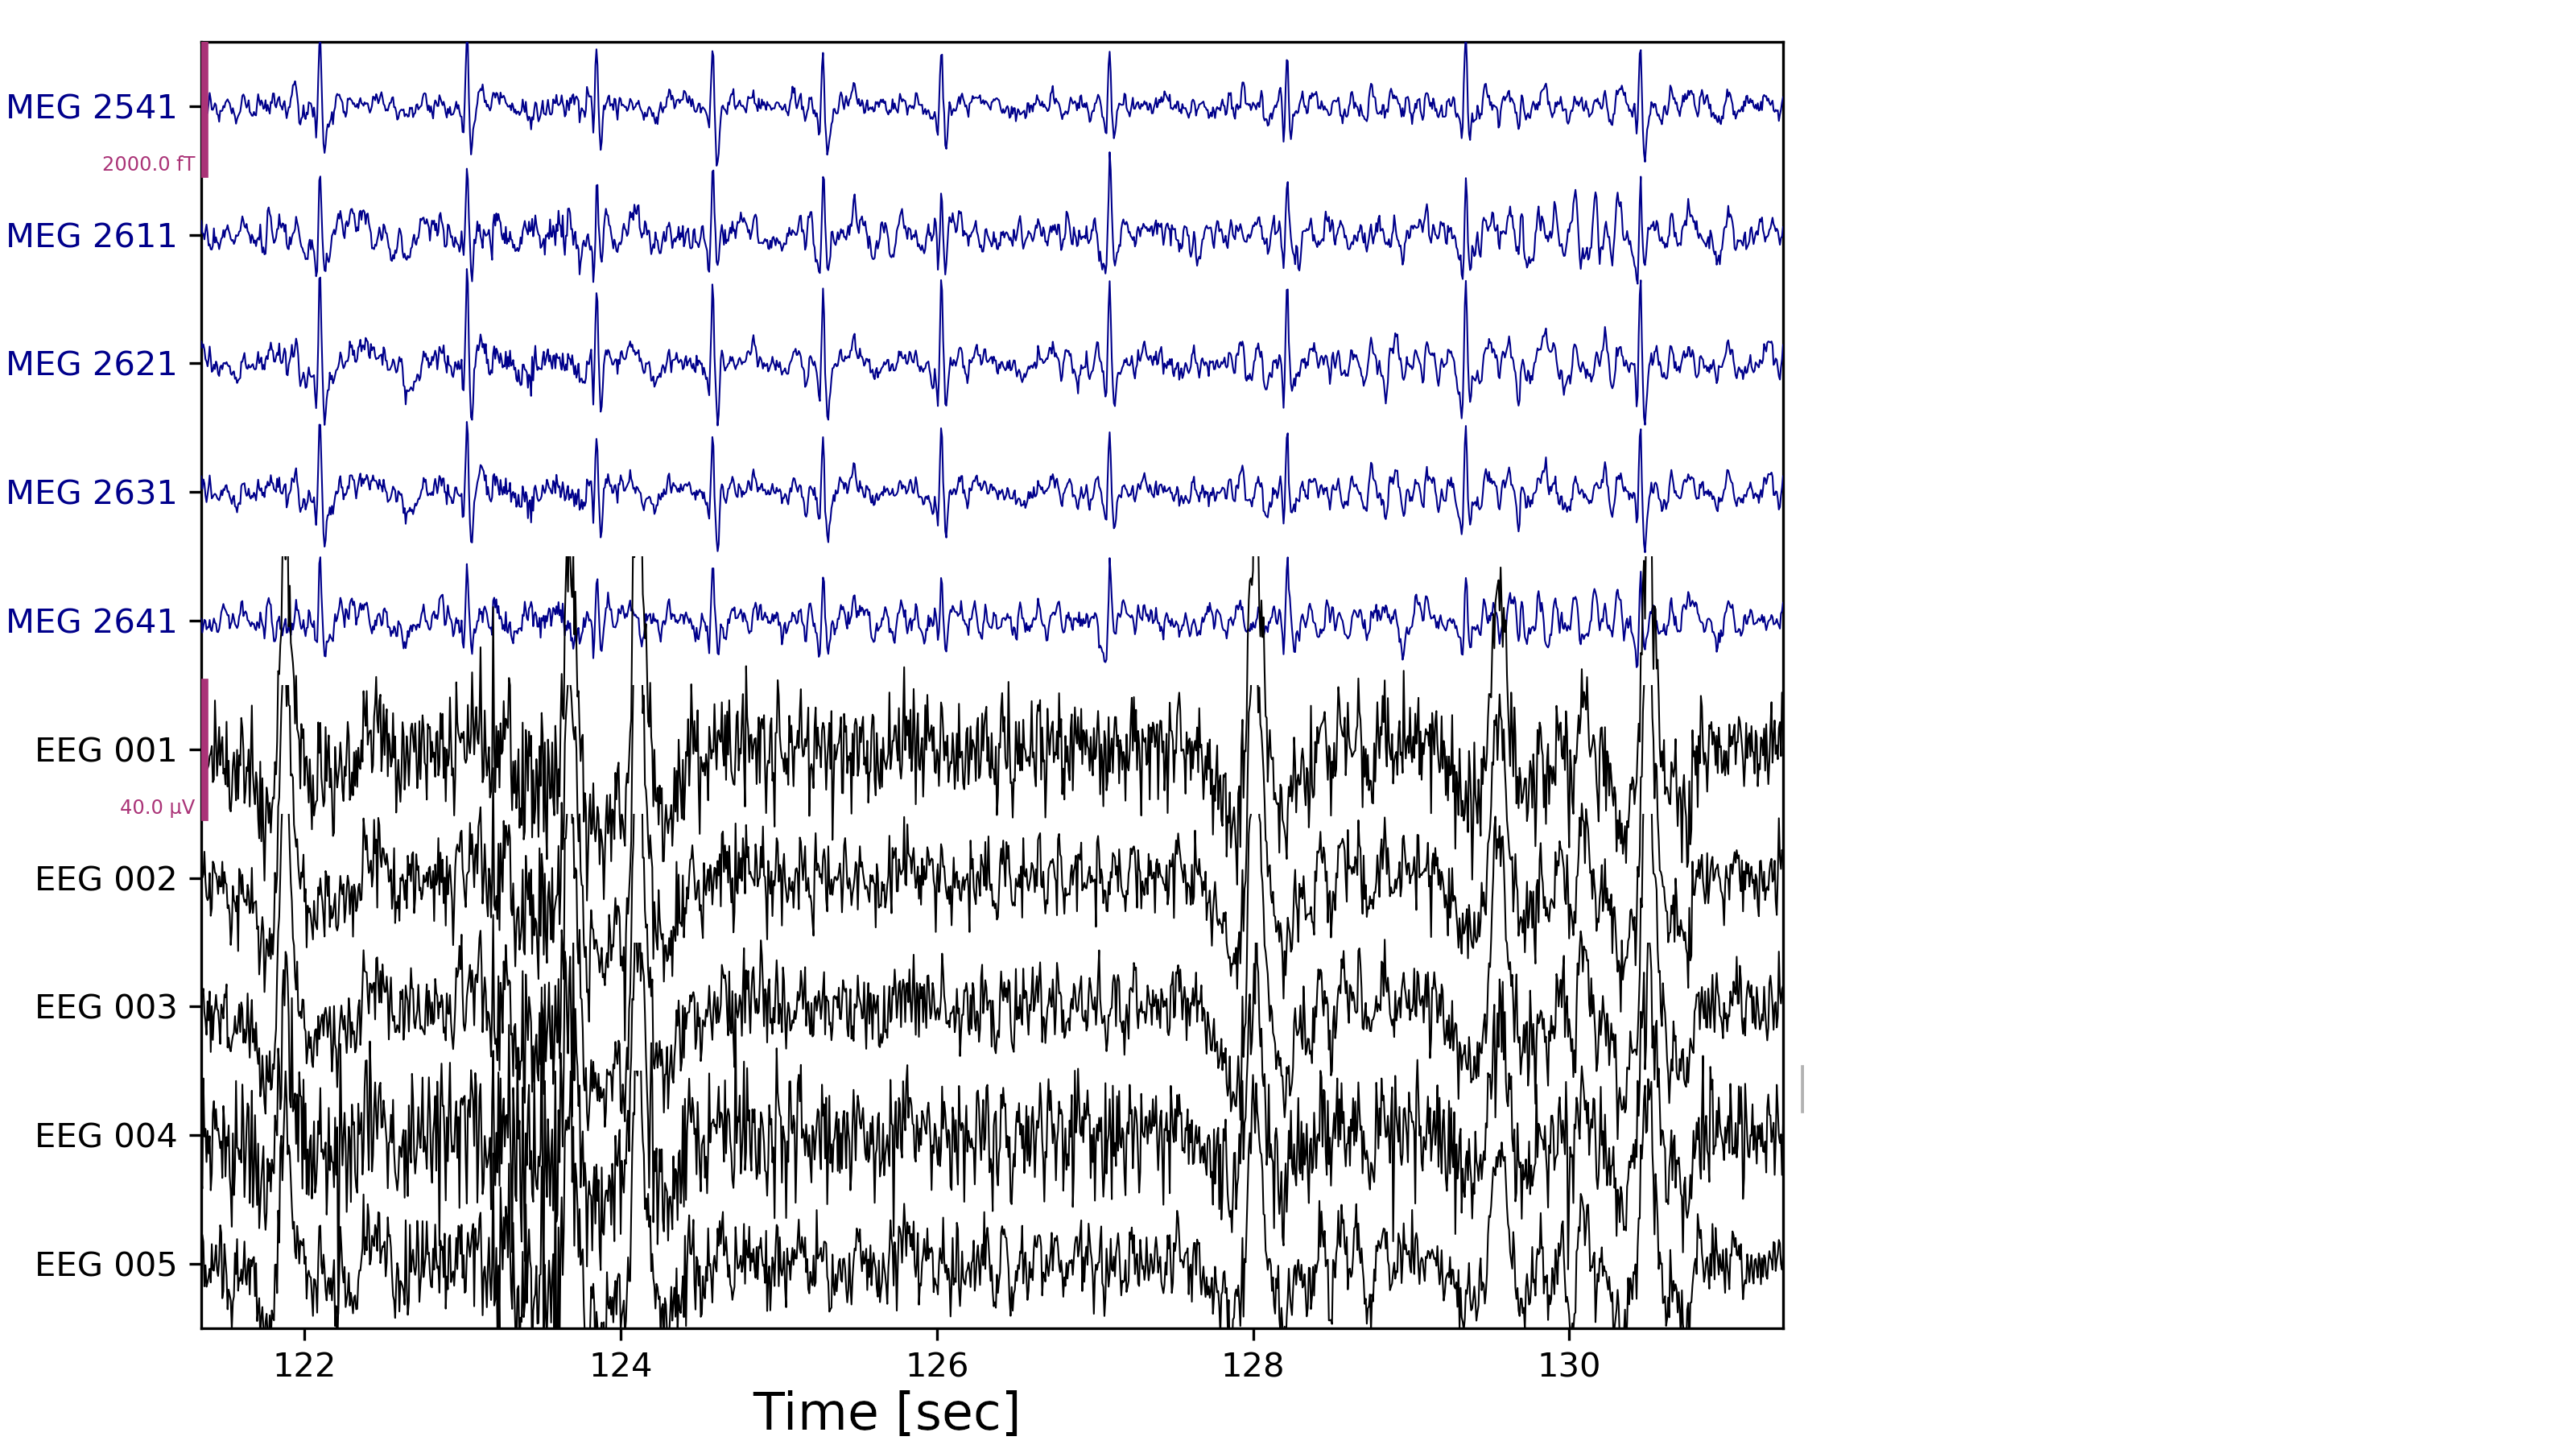
\includegraphics[width=.9\textwidth]{meeg_data_preproc}
        }
    }\\[1em]
    \begin{columns}
        \techterm{Noisy}%
        \techterm{Many artifacts}%
        \techterm{Complex}%
    \end{columns}
}

\frame{
    \frametitle{How to get back to electrical activity?}

    \definecolor{Z}{RGB}{45,162,65}
    \definecolor{D}{RGB}{180,35,35}
    \def\varX{{\color{linkcolor} \pmb X}}
    \def\varZ{{\color{Z} \pmb \varepsilon}}
    \def\varD{{\color{D} \pmb G}}
    {\centering
    \begin{tikzpicture}
    \tikzset{
        %Define standard arrow tip
        >=stealth',
        %Define style for boxes
        varstyle/.style={
            rectangle,
            rounded corners,
            draw=black,
            text width=1em,
            minimum height=1.5em,
            text centered},
    }
    \node (meg) {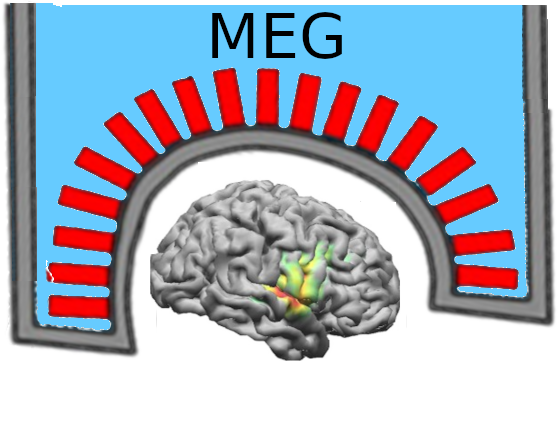
\includegraphics[width=12em]{meg_localised_source}};
    \draw[->, thick] ($(meg.east) - (0, 1.5em)$) -- ++(8em, 0)
    node[midway, align=center] (maxwell) {Maxwell's\\Equations}
    node[right] (topomap) {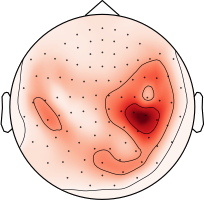
\includegraphics[width=6em]{topomap_somato}};
    \node[varstyle, below=.5em] at (topomap.south) (varX) {$\varX$};
    \node[below=0em of varX.south] {\bf Observed signal};
%        \draw[->, thick] (topomap.east) -- ++(5em, 0)
%        node[midway, align=center] {\small Problème\\ \small inverse}
    \node[varstyle, below=.2em of meg]
        (varZ) {$\varZ$};
        \node[below=0em of varZ.south] {\bf Electrical activity};
    \node[varstyle, below=3.8em of maxwell.center]
        (varD) {$\varD$};

    \uncover<2->{
         \draw[<-, thick] (meg.east) to[bend left, looseness=1]
            node [midway, above] {Inverse Problem}
            ($(topomap.west) + (0, 1.5em)$);
    }
    \end{tikzpicture}}
    \vskip0em
    {\bf Forward model: }$\varX{} = \varD\varZ$
    \hskip3em
    \uncover<2->{{\bf Inverse problem:} $\varZ = f(\varX)$ (ill-posed)}\\[1em]
    \uncover<3->{\centering
        \myitem{} Dipole fit
        \hskip2em
        \myitem{} Regularized optimization
        \hskip2em
        \myitem{} Deep-learning\\
        \mycite{Sarvas1987}\hskip2em
        \mycite{Gramfort2012}\hskip2em
        \mycite{Hecker2021}
    }

}

\frame{
    \frametitle{}

    \begin{columns}[c]
        \column{.6\columnwidth}
    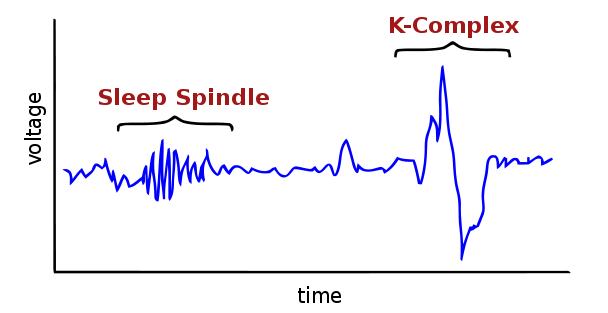
\includegraphics[width=\textwidth, trim={6em 6em 0 0}, clip]{sleep_spinddle}
        \column{.35\columnwidth}
            \highlightbox{
                \centering \Large
                Neural signals exhibit
                diverse and complex
                morphologies
            }
    \end{columns}
    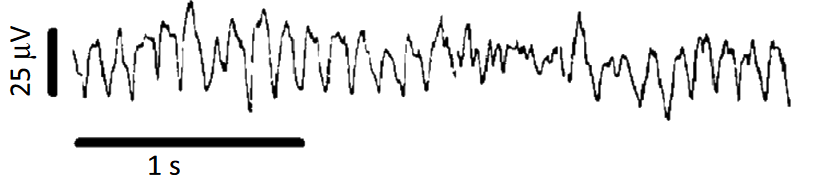
\includegraphics[width=\textwidth]{mu_rythm}\\[-1.5em]
    \rightcite{Cole \& Voytek 2017}
    \vskip-7em
        \begin{columns}[c]
        \column{.75\columnwidth}
        \visible<2->{\highlightbox{\vskip.1em
        \Large Waveform shape can be related to diseases\\
        \eg{} Parkinson \rightcite{Jackson et al. 2019}}\\[.3em]}
        \end{columns}
    \vskip3em
    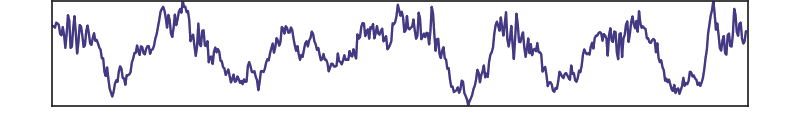
\includegraphics[width=\textwidth]{cfc}\\[-.8em]
    \rightcite{\footnotesize Dupré la Tour et al. 2017}
}

\frame{
    \frametitle{Repeated Stimuli -- Evoked Response \rightcite{Gramfort et al. 2013}}

    \myitem{} Subject is presented some stimuli -- Audio, Visual, Motor, ...\\[.5em]
    \myitem{} Record onset of the stimuli\\[.5em]
    \myitem{} Average signal on window aligned around the stimulus\\[1em]

    \begin{columns}

        \column{.3\textwidth}
        \centering
        Evoked response to an auditory stimuli\\[.5em]
        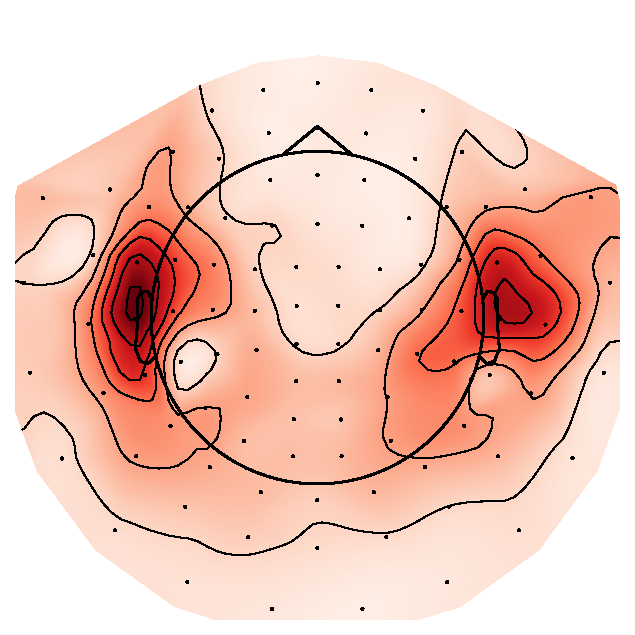
\includegraphics[width=.8\textwidth]{evoked_topo}
        \column{.6\textwidth}
        {\centering
            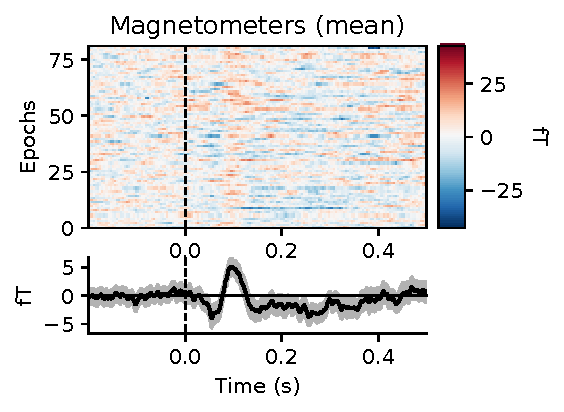
\includegraphics[width=\textwidth]{evoked_response}\\
        }
    \end{columns}
    \rightcite{MNE-Python}
}

\frame{
    \frametitle{Repeated Stimuli -- Induced Response \rightcite{Gramfort et al. 2013}}

    \myitem{} Subject is presented some stimuli -- Audio, Visual, Motor, ...\\[.5em]
    \myitem{} Average PSD on window aligned around the stimulus\\
    \rightcite{MNE-Python}\\[-.5em]

        \centering
        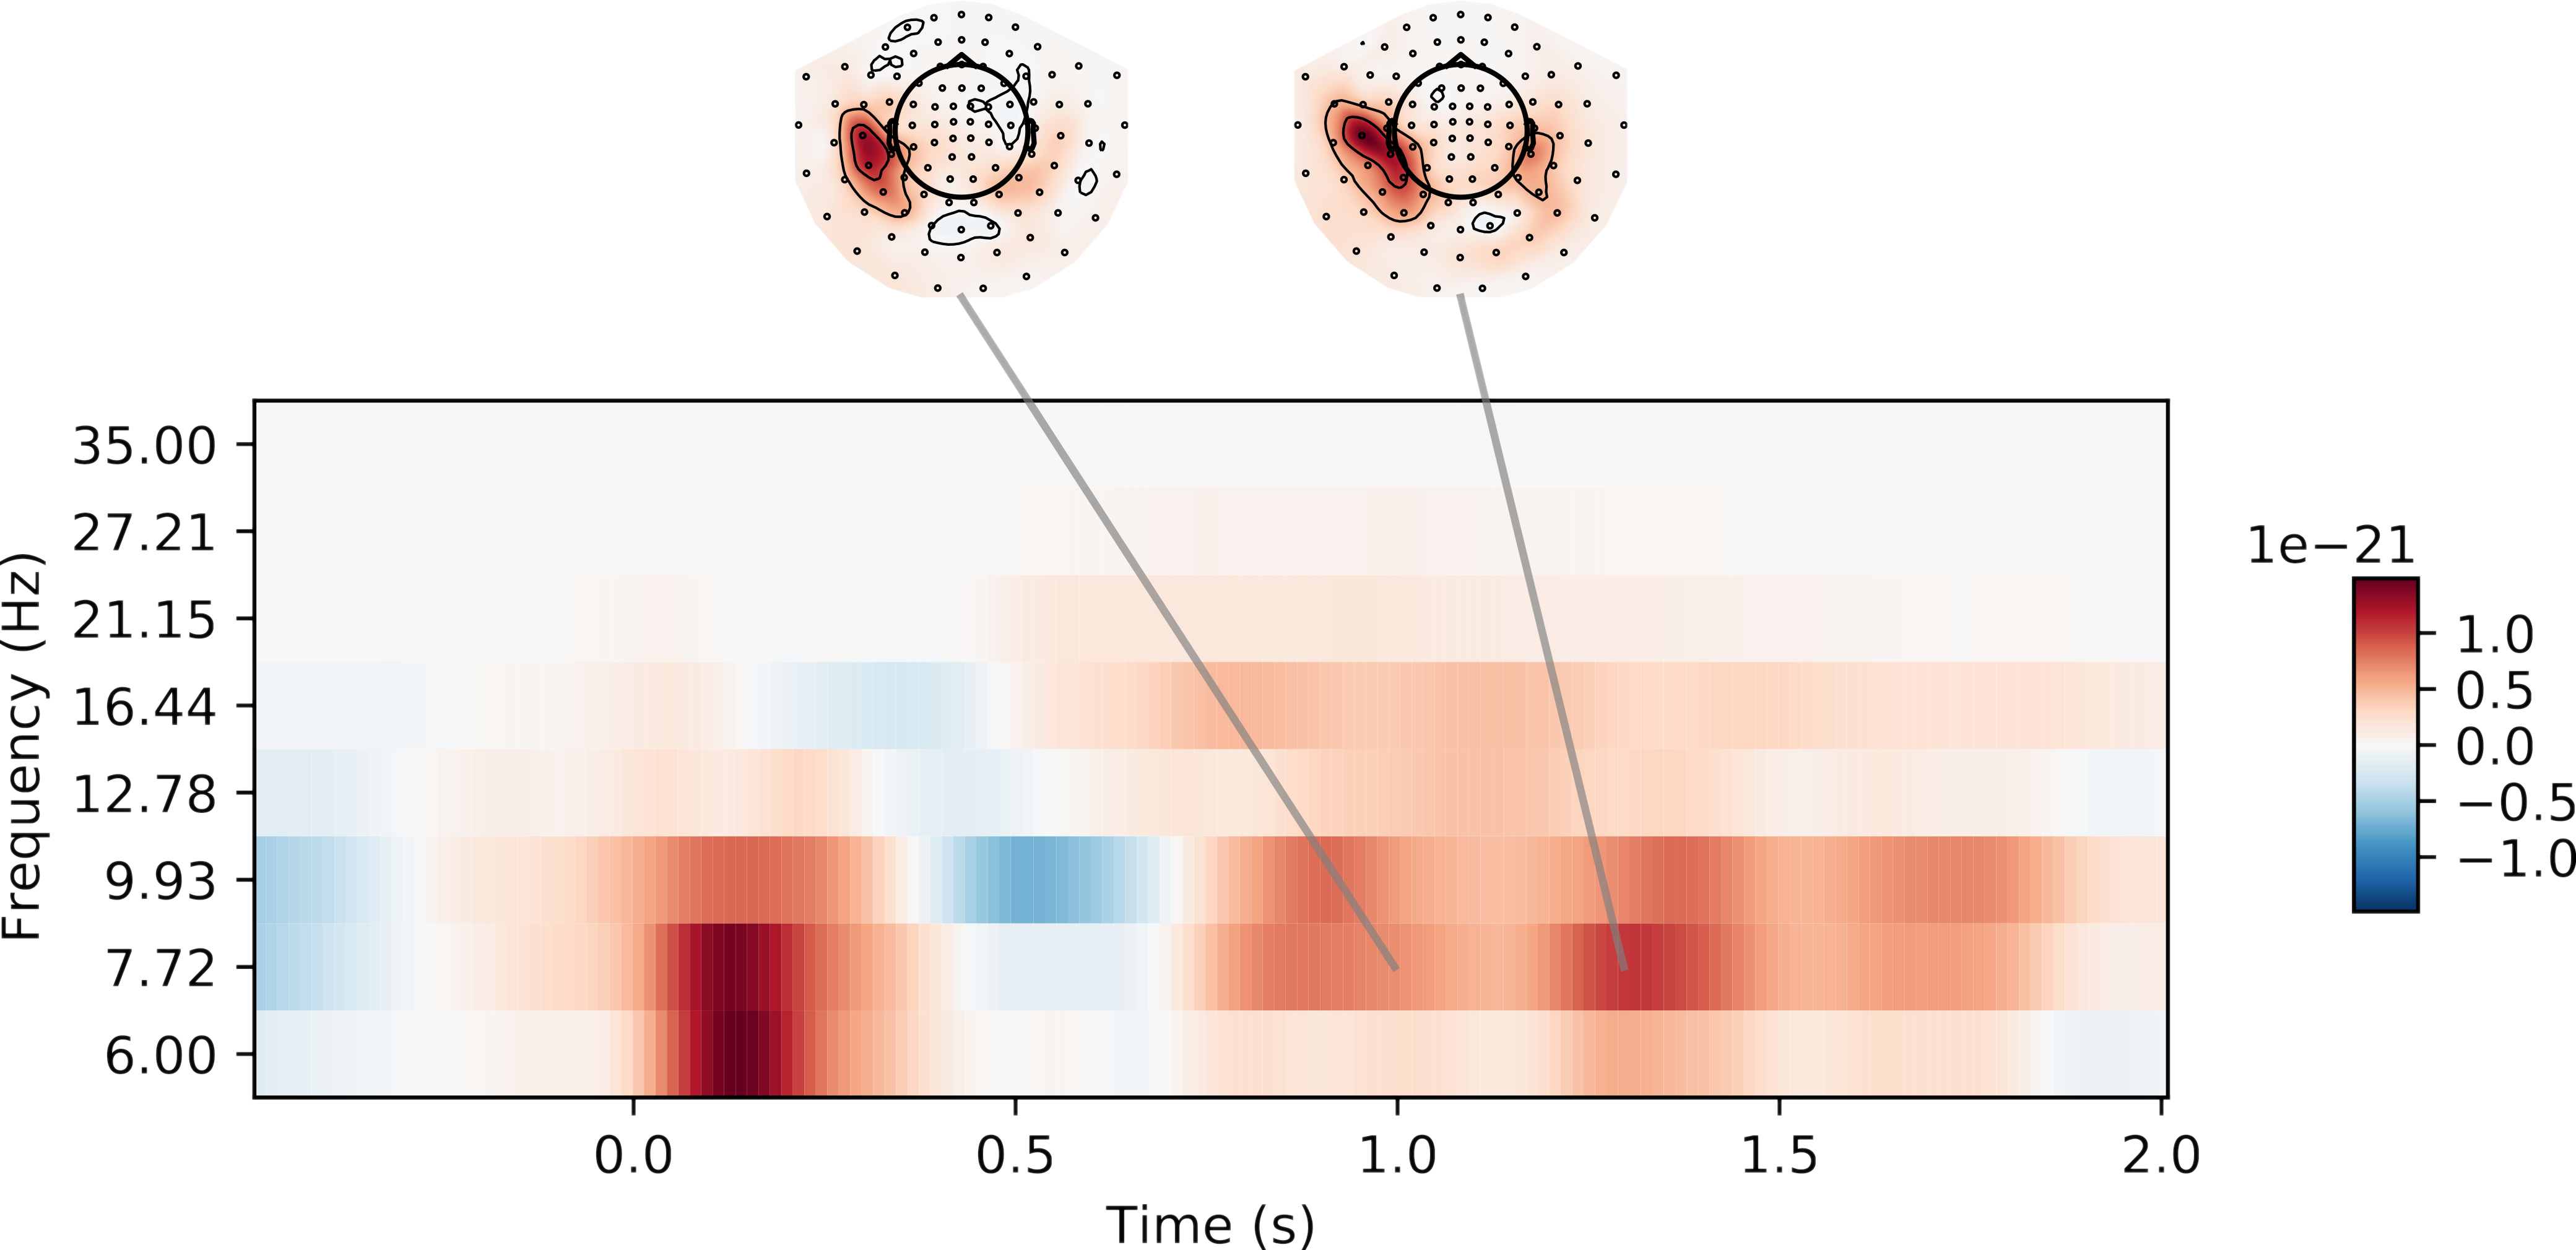
\includegraphics[width=\textwidth]{somato_time_freq.png}\\[.1em]
        Evoked response to an somatosensory stimuli\\

}

% \frame{
%     \frametitle{Learning the waveform}


%     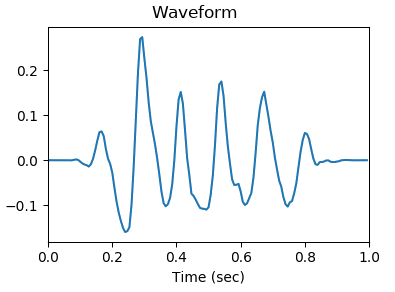
\includegraphics[width=.5\textwidth]{mu_waveform}%
%     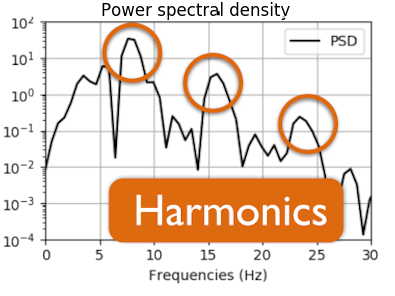
\includegraphics[width=.5\textwidth]{mu_waveform_harmonic}

%     \visible<2>{
%     \strongpoint{Can we actually learn the waveform and relate them to stimuli?}}
% }


% \frame{
%         \frametitle{``Textbook'' brain rythms}

%         \centering
%         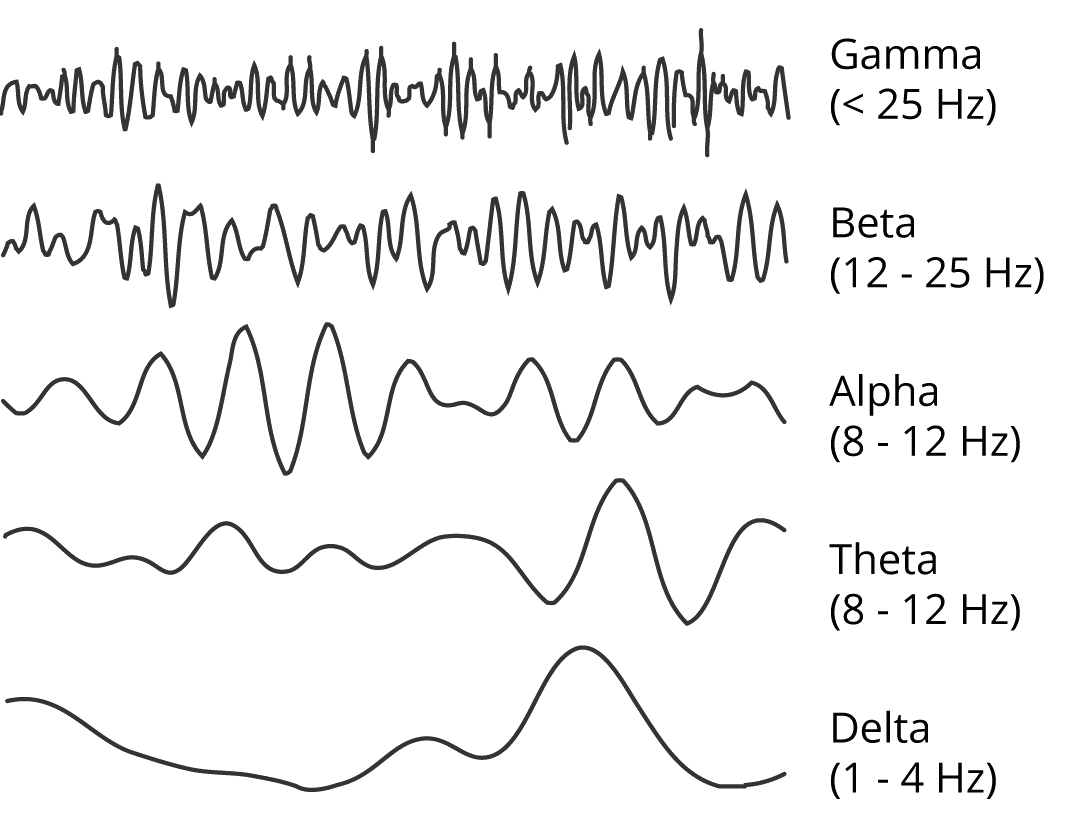
\includegraphics[width=.8\textwidth]{brain_rythm}

% }




% \frame{
%     \frametitle{Linear filtering}

%     After Linear filters, everything looks like a sinusoïd.
%     {\centering
%     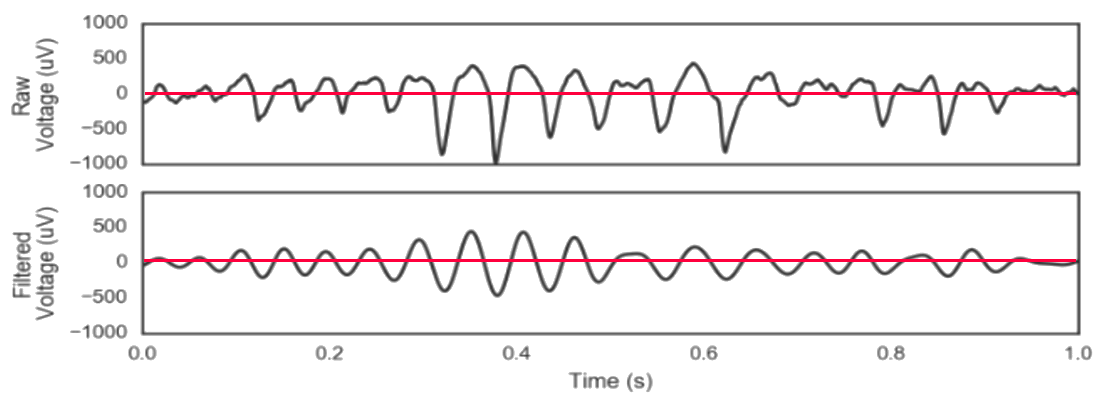
\includegraphics[width=.9\columnwidth]{filtering_mu_waves}\\[1em]
%     \strongpoint{Lose the asymmetry and the shape information}
%     }

% }

% \frame{
%     \frametitle{Fourier Fallacy}
%     \large
%     {\centering
%     "Even though it may be possible to analyze the complex forms of brain waves into a {\bf number of different sine-wave} frequencies, this may lead only to what might be termed a “{\bf Fourier fallacy}”, if one assumes {\bf ad hoc} that all of the necessary frequencies actually occur as periodic phenomena in {\bf cell groups} within the brain."\\[.5em]}
%     \mycite{Jasper1948}
%     \vskip.5em
%     \visible<2->{
%         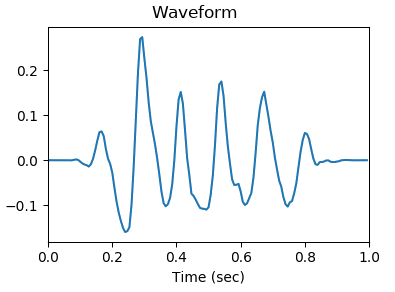
\includegraphics[width=.5\textwidth]{mu_waveform}%
%         \alt<3>{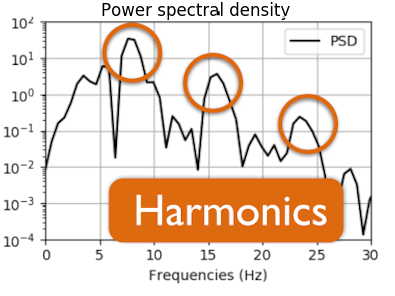
\includegraphics[width=.5\textwidth]{mu_waveform_harmonic}}
%                {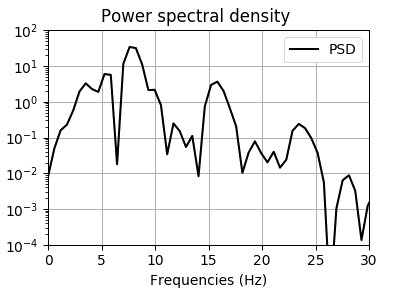
\includegraphics[width=.5\textwidth]{mu_waveform_psd}}
%     }

% }

\section{Learning the waveform:\\Convolutional Dictionary Learning}
\parttitleframe{Grosse2007}

\frame[t]{
	\frametitle{Local structure in signals}

	\visible<5->{
		\textbf{Key idea}: decouple the localization of the
							patterns and their shape}
    \vskip.5em%
    \centering%
    \only<1>{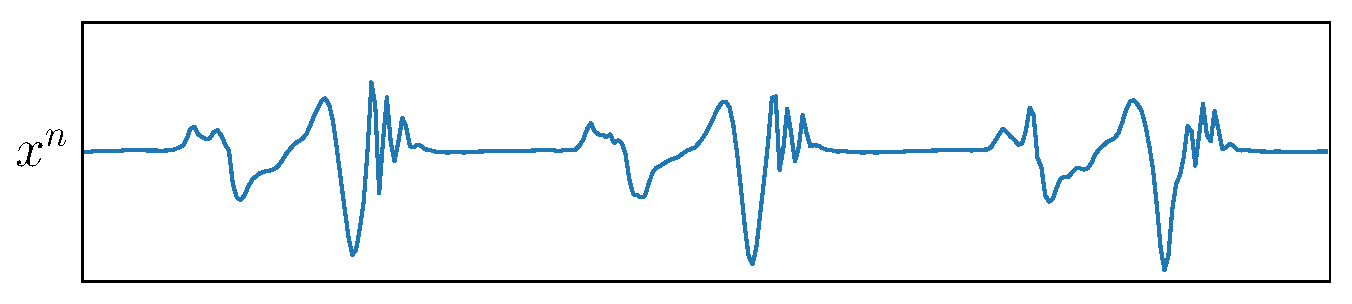
\includegraphics[width=\textwidth]{intro_csc_0}}%
    \only<2>{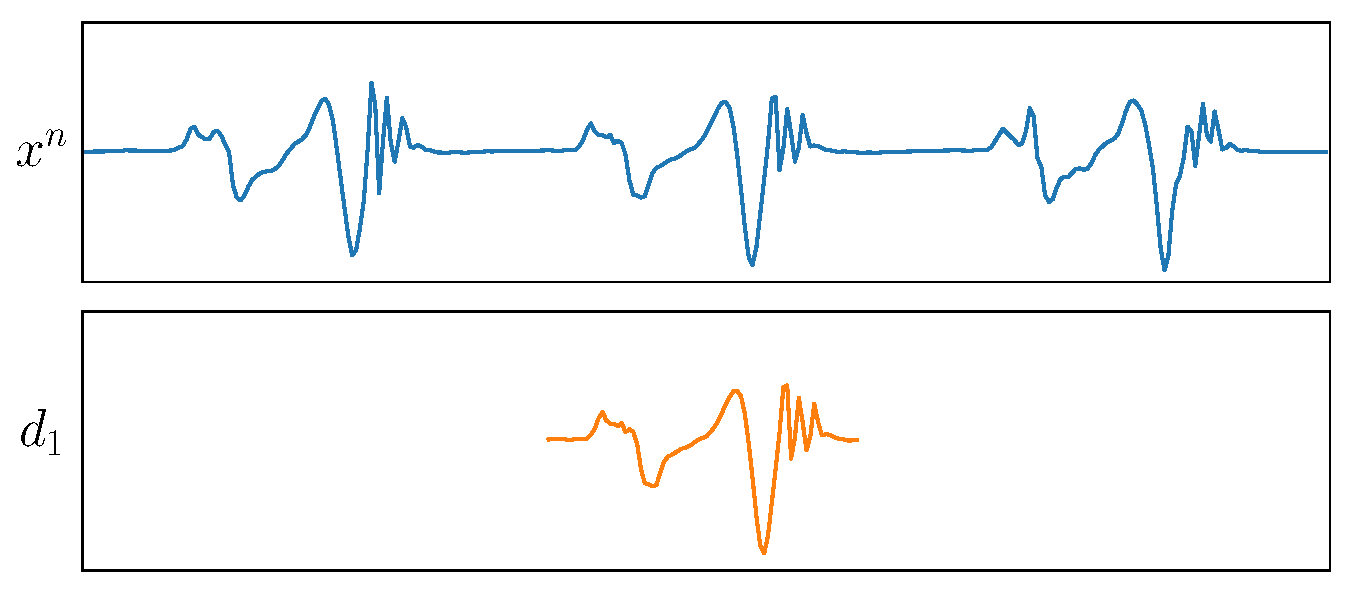
\includegraphics[width=\textwidth]{intro_csc_1}}%
    \only<3>{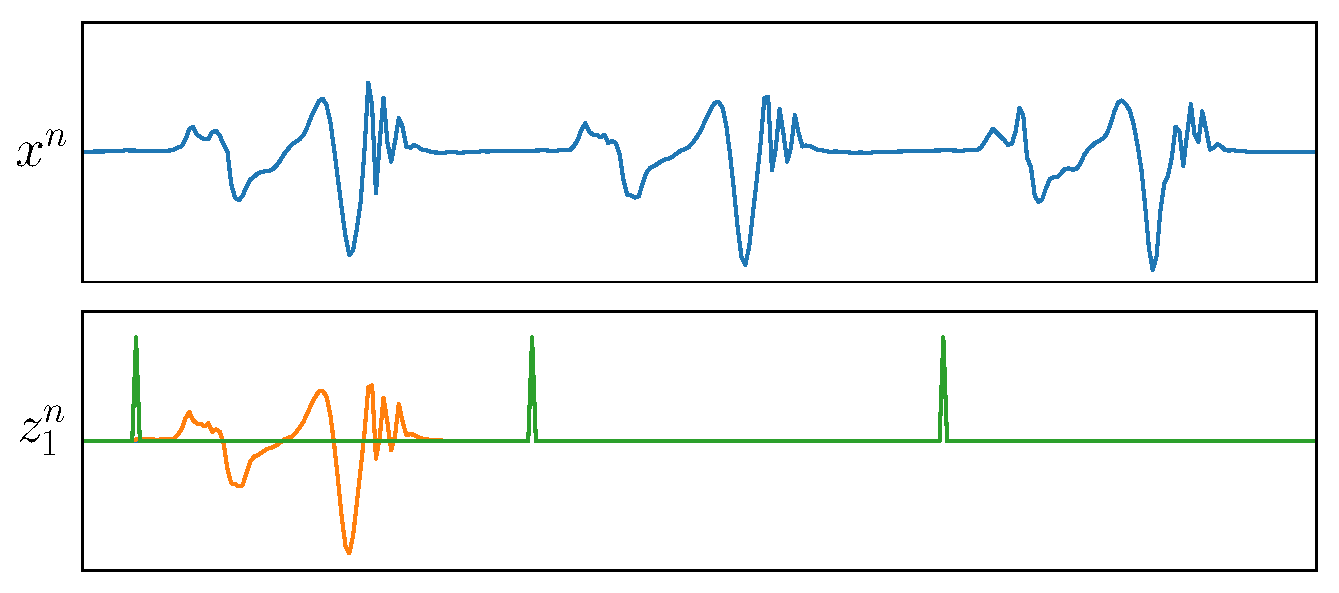
\includegraphics[width=\textwidth]{intro_csc_2}}%
    \only<4>{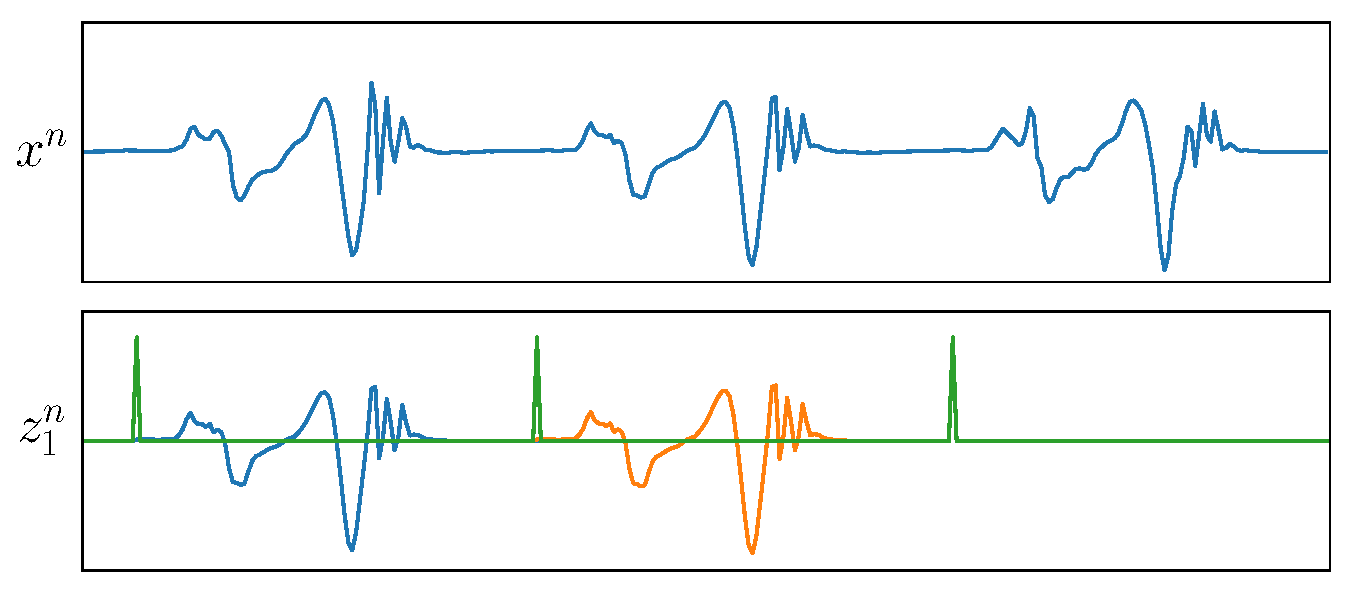
\includegraphics[width=\textwidth]{intro_csc_3}}%
    \only<5>{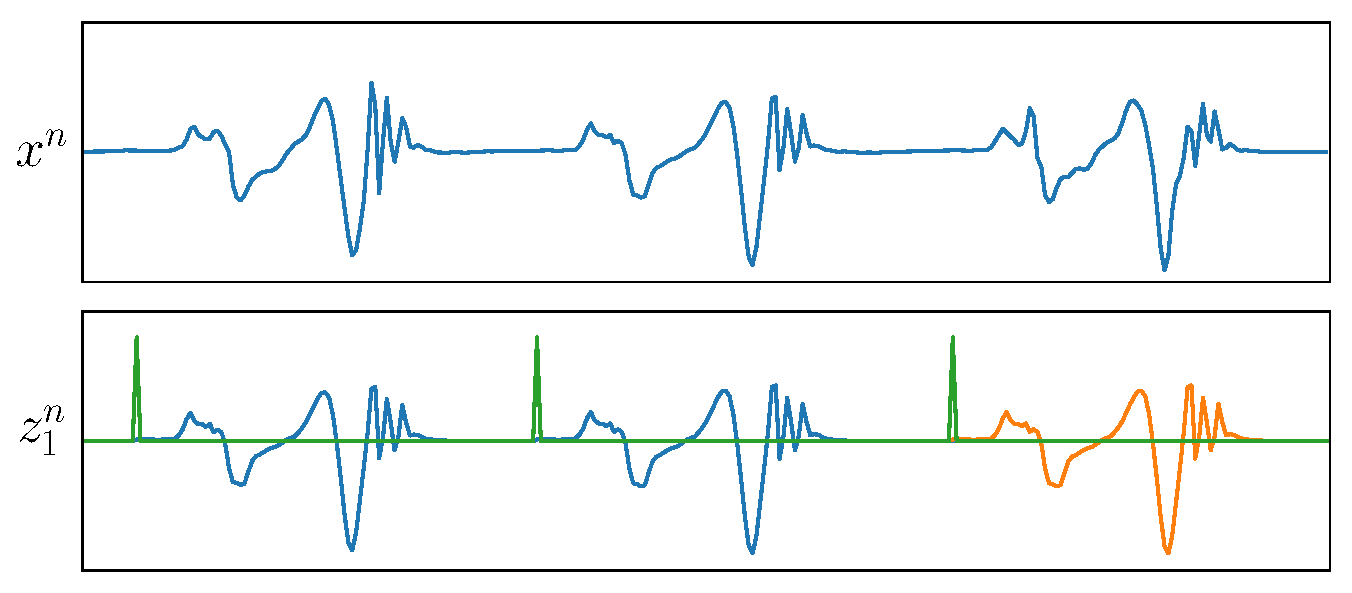
\includegraphics[width=\textwidth]{intro_csc_4}}%
    \only<6->{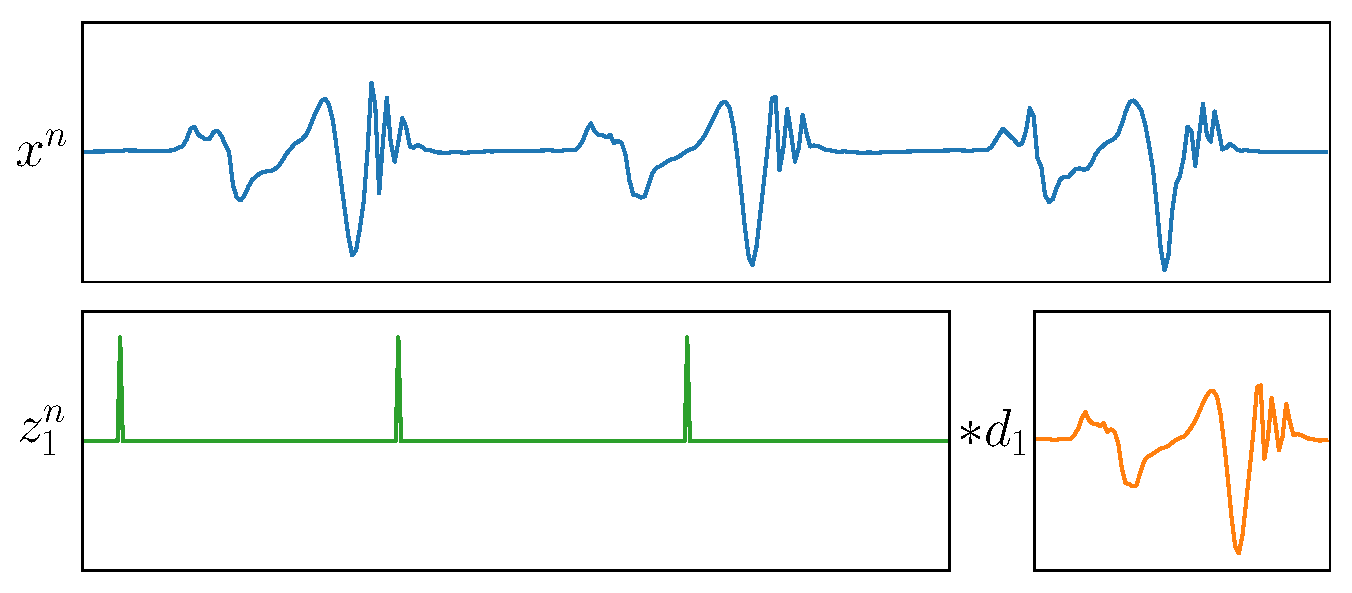
\includegraphics[width=\textwidth]{intro_csc_5}}%
    \vskip0em%
    \only<7>{%
        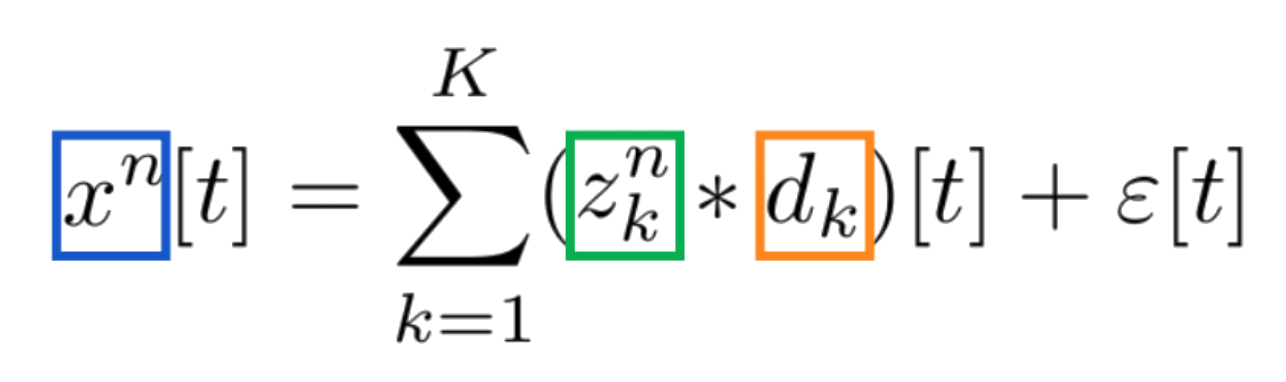
\includegraphics[width=.6\textwidth]{csc_explain_eq_color}%
    }
}

\frame{
    \frametitle{Convolutional Dictionary Learning \mycite{Grosse2007}}

    For a set of $N$ univariate signals $x^n$, solve\\[.5em]
        {\centering 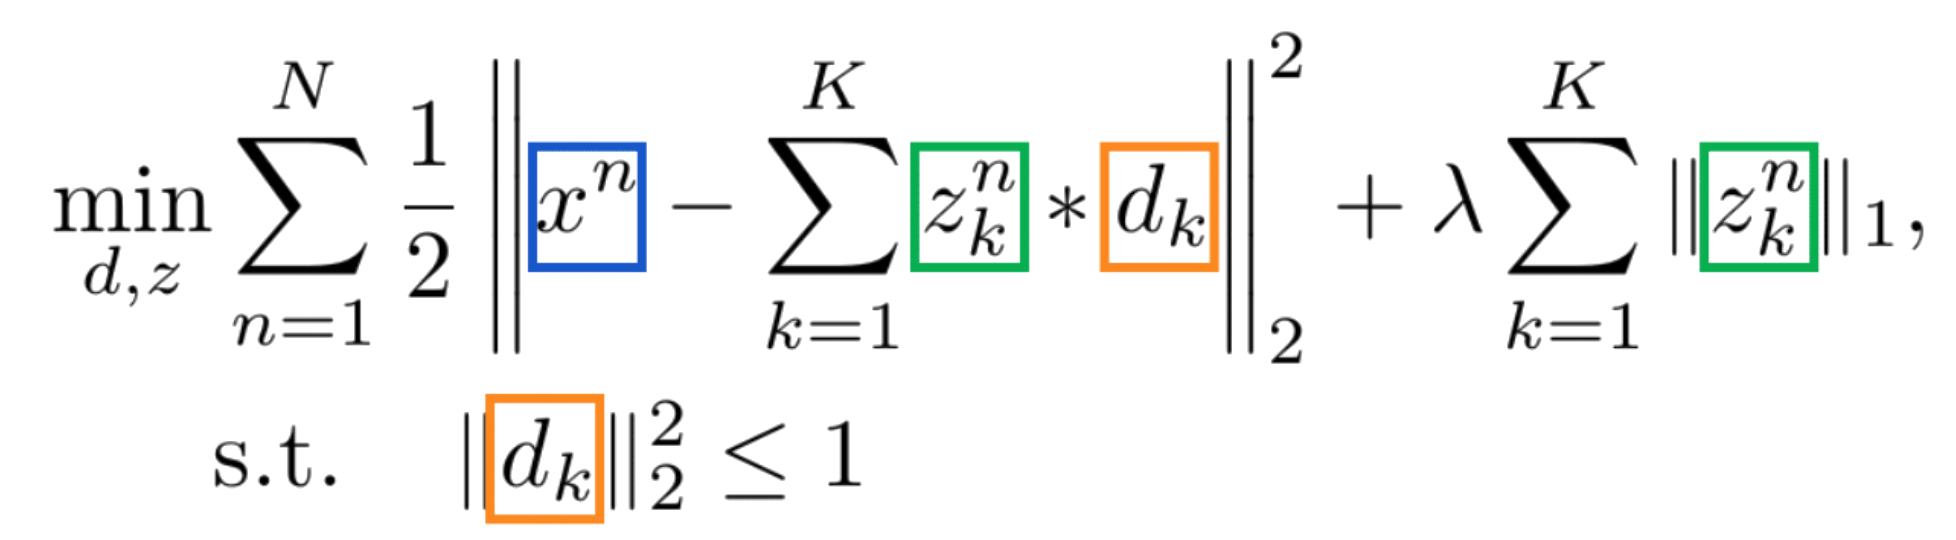
\includegraphics[width=.8\textwidth]{csc_eq_l1}\\[1em]}
    \textbf{Hypothesis:} patterns $d_k$ are not present everywhere in the signal. They are localized in time.
    \strongpoint{Sparse activation signals $z$}
    \vskip2em
    \textbf{Technical hypothesis:} the patterns are in the $\ell_2$-ball: $\|d_k\|_2^2 \le 1$.
}


\frame{
    \frametitle{Optimization strategy}
    \textbf{Bi-convex:} The problem is not jointly convex in $z^n_k$, and  $d_k$
    but it is convex in each block of coordinate.\\[1em]

    \textbf{Alternate minimization} (\emph{a.k.a.} Bloc Coordinate Descent):\\[.5em]

    \begin{itemize}\itemsep.5em
    \item \textbf{Z-step:} given a fixed estimate of the atom, compute the activation signal $z^n_k$ associated to each signal $x^n$.
    \item \textbf{D-step:} given a fixed estimate of the activation, update the atoms in the dictionary $d_k$.
    \end{itemize}

    \vskip1em
    \pause
    \textbf{Unrolled optimization}:\\[.5em]

    \begin{itemize}\itemsep.5em
    \item \textbf{Z-step:} use an fixed differentiable procedure $f(x^n, D)$.
    \item \textbf{D-step:} learn $D$ through back-propagation.
    \end{itemize}
    \rightcite{Malezieux et al. 2022}
}

\begin{frame}{How to extend CSC to multivariate signals?}
    We can just use multivariate convolution,
    \[
        \underbrace{X[t]}_{\in\Rset^P} = \sum_{k=1}^K \left(z_k * D_k\right)[t] = \sum_{k=1}^K \sum_{\tau=1}^L z_k[t-\tau] \underbrace{D_k[\tau]}_{\in \Rset^P}
    \]
    with:
    \begin{itemize}
        \item $X$ a multivariate signal of length $T$ in $\Rset^P$
        \item $D_k$ a multivariate signal of length $L$ in $\Rset^P$
        \item $z_k$ a univariate activation signal of length $\tT = T - L + 1$
    \end{itemize}
    \vskip1em
    However, this model does not account for the physics of the problem.
    \end{frame}


\section{Rank-1 constrained dictionary learning}
\parttitleframe{DuprelaTour2018}


\begin{frame}{EM wave diffusion}
	\begin{itemize}
		\uncover<1->{\item Recording here with 8 sensors}
		\uncover<2->{\item EM activity in the brain}
		\uncover<3->{\item The electric field is spread \textbf{linearly} and \textbf{instantaneously} over all sensors (Maxwell equations)}
	\end{itemize}
	\centering
	\only<1>{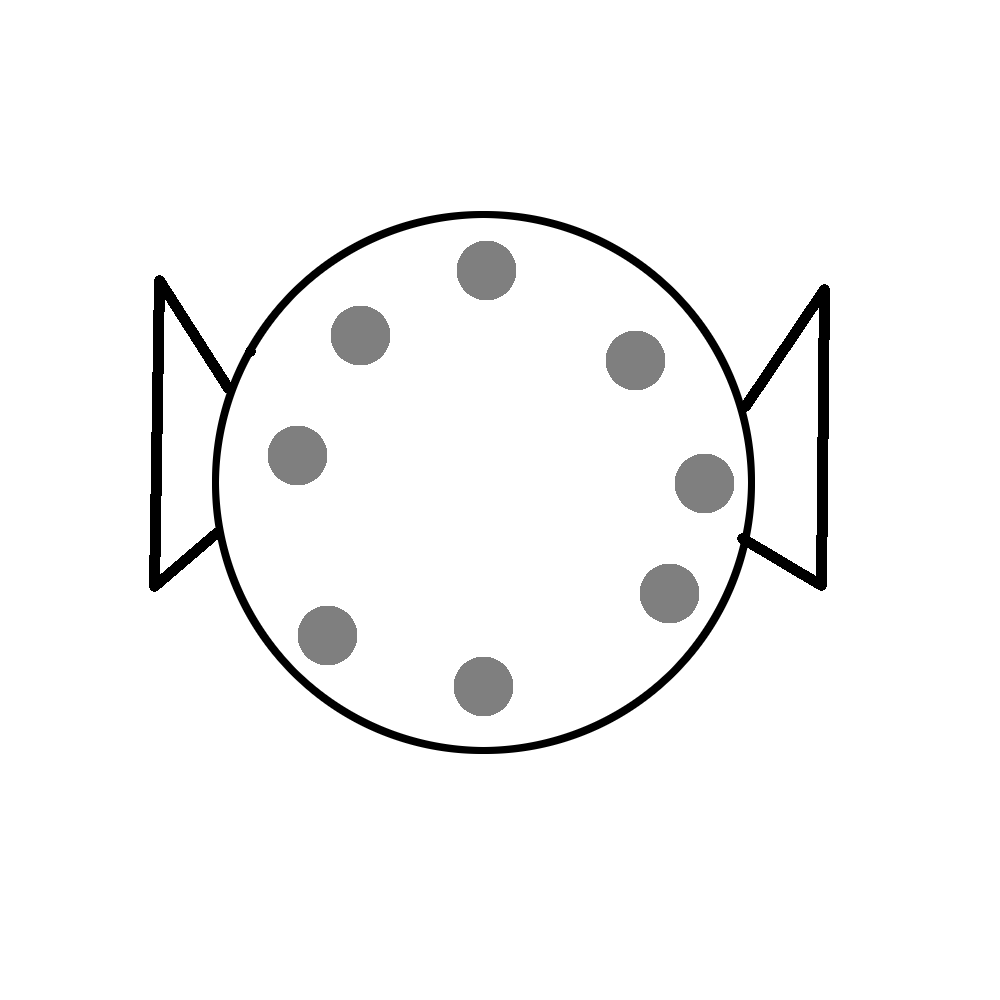
\includegraphics[width=.5\textwidth]{physic1}}%
	\only<2>{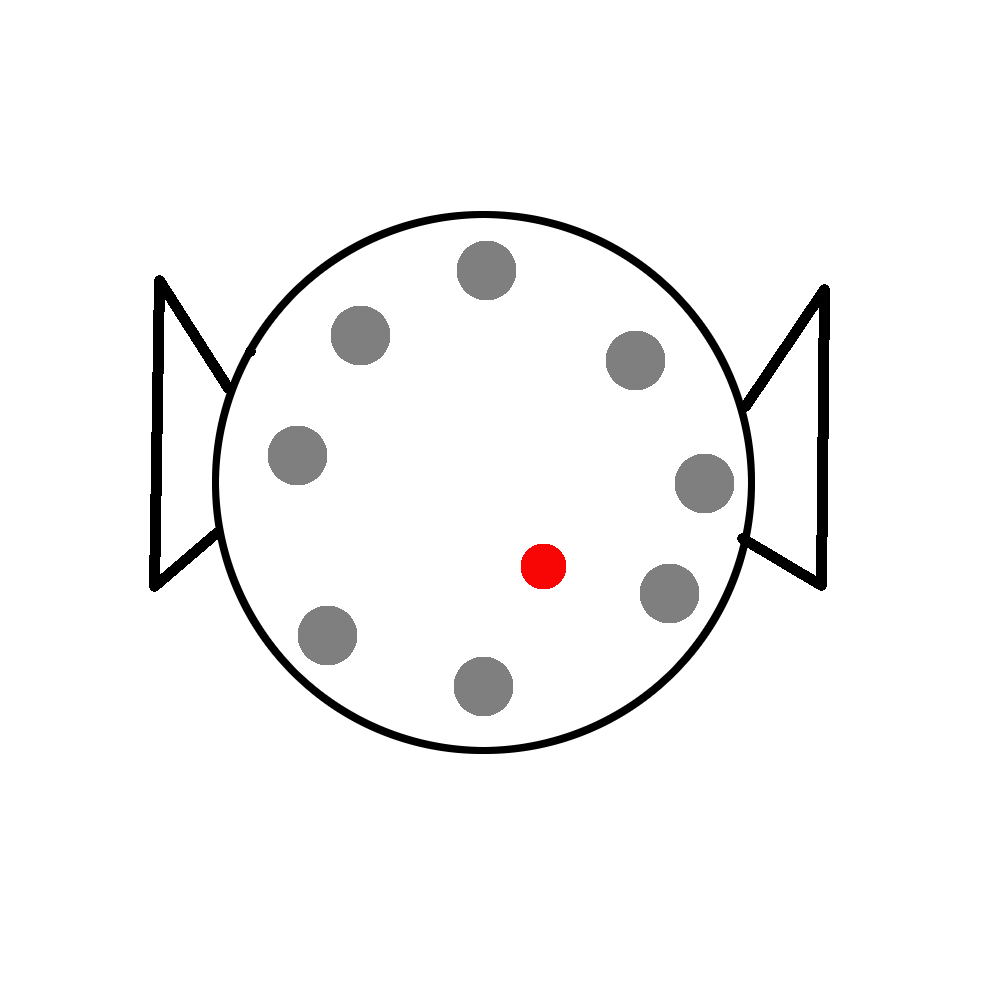
\includegraphics[width=.5\textwidth]{physic2}}%
	\only<3>{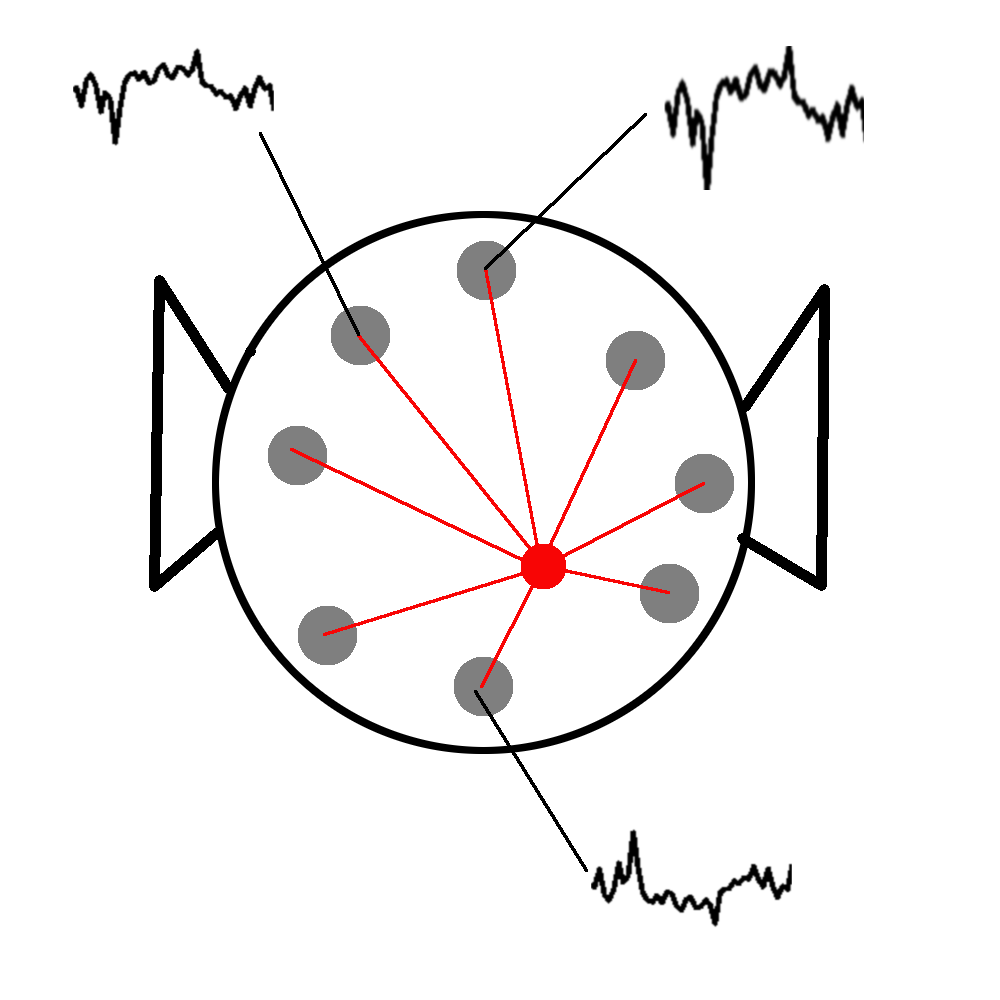
\includegraphics[width=.5\textwidth]{physic3}}%
	\only<4>{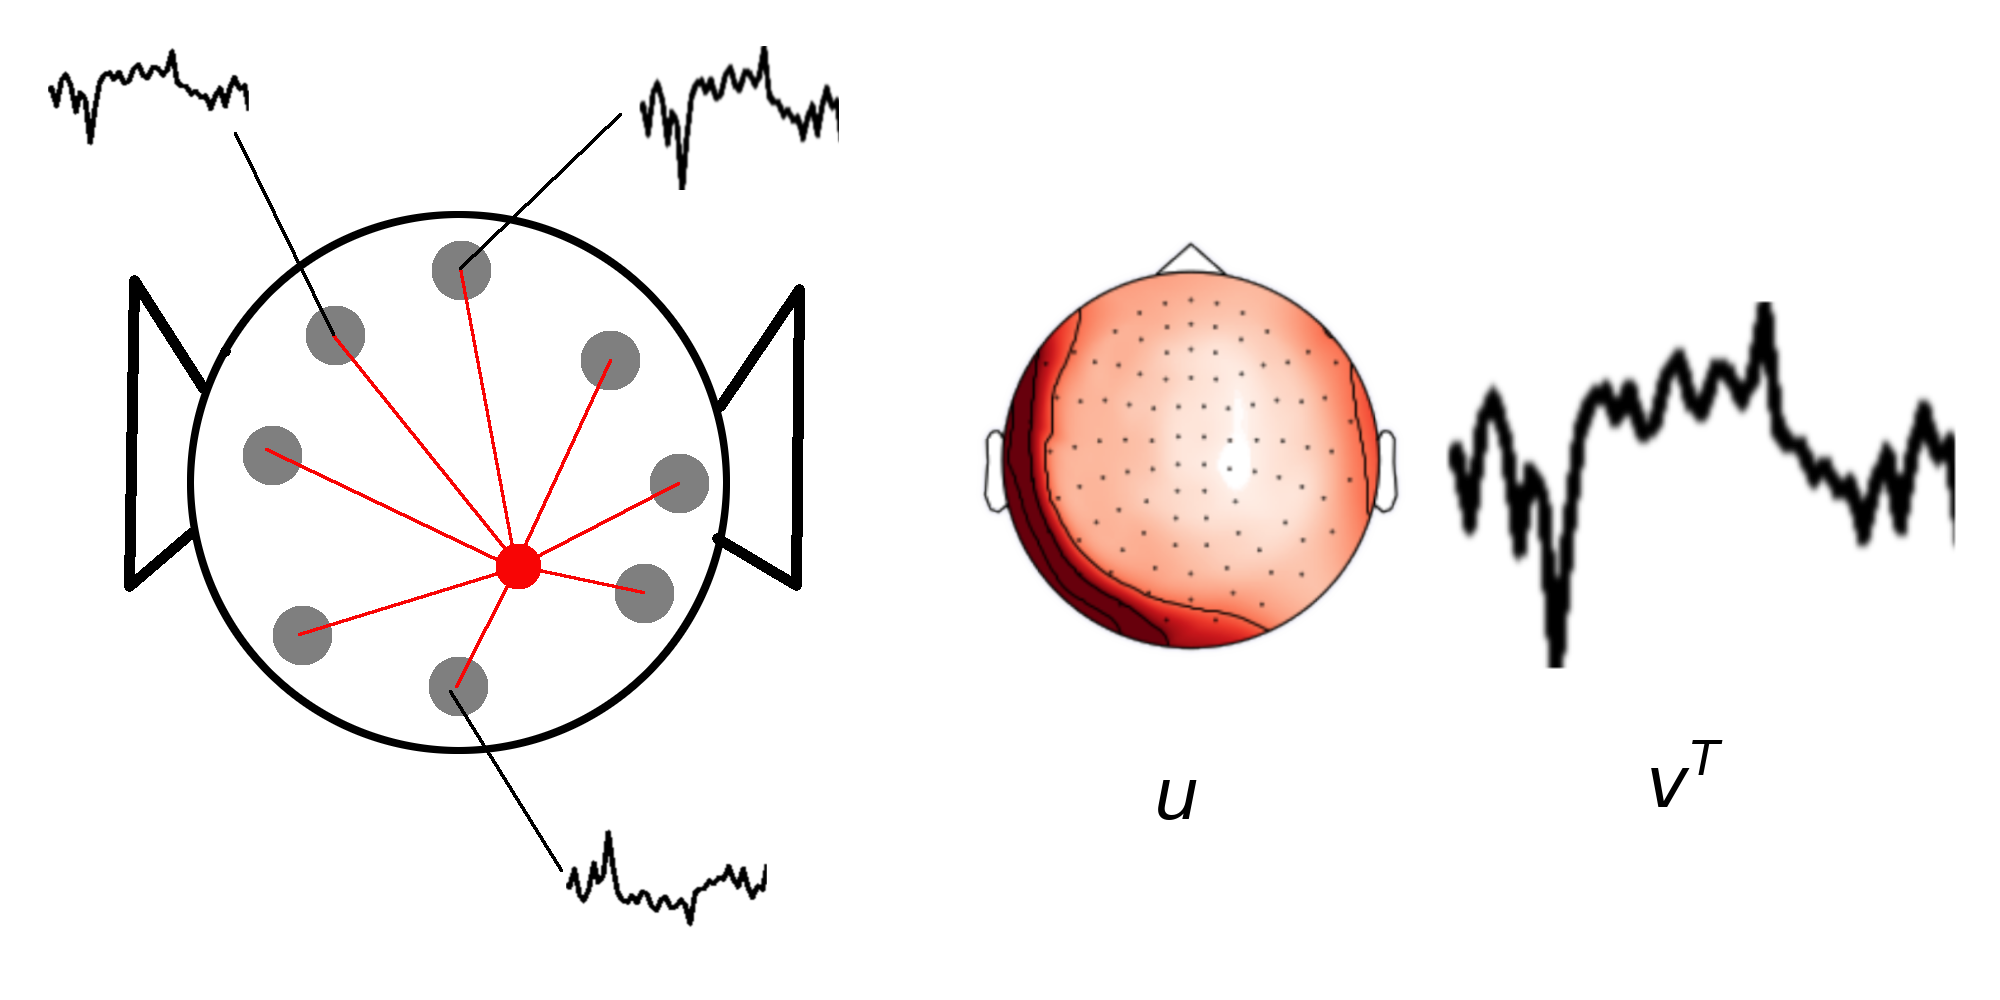
\includegraphics[width=\textwidth]{physic4}}
\end{frame}

\begin{frame}{Multivariate CSC with rank-1 constraint}
	\textbf{Idea}: Impose a rank-1 constraint on each dictionary atom $D_k$
	\vskip1em
	To make the problem tractable, use $u_k$ and $v_k$ \st{} $D_k = u_kv_k^\top$.

	\begin{equation}
	\label{eq:multichannel_csc}
	\begin{split}
	\min_{u_k, v_k, z_k^n} &\sum_{n=1}^N\frac{1}{2}\left\|X^n - \sum_{k=1}^K z^n_k * (u_k^{ } v_k^\top)\right\|_{2}^{2}
	+ \lambda  \sum_{k=1}^K \left\|z^n_k\right\|_1, \hspace{6pt}\\
	&\text{s.t. } ~~ \|u_{k}\|_2^2 \leq 1 \text{  , }\|v_{k}\|_2^2 \leq 1 \text{  and } z_k^n \geq 0~.
	\end{split}
	\end{equation}

	Here,
	\begin{itemize}
		\item $u_k \in \Rset^P$ is a spatial pattern
		\item $v_k \in \Rset^L$ is a temporal pattern
	\end{itemize}

    \strongpoint{This is a tri-convex problem}
\end{frame}



% \begin{frame}{Optimization strategy}
% \textbf{Tri-convex:} The problem is not jointly convex in $z^n_k$, $u_k$ and $v_k$ but it is convex in each block of coordinate.\\[1em]

% We can use a block coordinate descent, aka alternate minimization, to converge to a local minima of this problem. The 3 following steps are applied alternatively:

% \begin{itemize}
% 	\item \textbf{Z-step:} given a fixed estimate of the atom, compute the activation signal $z^n_k$ associated to each signal $X^n$.
% 	\item \textbf{u-step:} given a fixed estimate of the activation and temporal pattern, update the spatial pattern $u_k$.
% 	\item \textbf{v-step:} given a fixed estimate of the activation and spatial pattern, update the temporal pattern $v_k$.
% \end{itemize}
% \end{frame}

\begin{frame}{Z-step: Locally greedy coordinate descent (LGCD)}

$N$ independent problem such that
\[
	\label{eq:sparse_code}
	\min_{z_k^n \ge 0} \frac{1}{2} \left\|X^n - \sum_{k=1}^K z_k^n * D_k\right\|_2^2
	+ \lambda\sum_{k=1}^K\left\|z_k^n\right\|_1~.
\]
This problem is convex in $z_k$ and can be solved with different techniques:
\begin{itemize}
	\item FISTA \mycite{Chalasani2013}
	\item ADMM \mycite{Bristow2013}
	\item L-BFGS \mycite{Jas2017}
	\item Greedy CD \mycite{Kavukcuoglu2010}
\end{itemize}

\strongpoint{These methods can be slow for long signals as the complexity of each iteration is at least linear in the length of the signal.}

\end{frame}

\begin{frame}[t]{Z-step: Locally greedy coordinate descent (LGCD)}

	{\bf Coordinate Descent:} only 1 coordinate is updated at each iteration:\\
	\vskip.5em
	\begin{enumerate} % [<+->]
        \itemsep2em
		\item The coordinate $z_{k_0}[t_0]$ is updated to its optimal value $z'_{k_0}[t_0]$\\when all other coordinate are fixed.
		\item The updated coordinate is chosen\\[1em]

        \begin{itemize}\itemsep.5em
            \item Cyclic: $\mathcal{O}(1)$ \mycite{Friedman2007}
            \item Randomized: $\mathcal{O}(1)$ \mycite{Nesterov2010}
            \item Greedy: $\mathcal{O}(K\widetilde{T})$ \mycite{Osher2009}\\
            by maximizing $|z_k[t] - z'_k[t]|$\\
            \item Locally Greedy: $\mathcal{O}(K\widetilde{L})$ \mycite{Moreau2018}\\
            by maximizing $|z_k[t] - z'_k[t]|$ on a window
        \end{itemize}
    \end{enumerate}

    % \only<1>{
    %     For convolutional CD, we can use optimal updates:
    %     $$
    %         Z'_{k_0}[\omega_0] = \frac{1}{\|\pmb D_{k_0}\|_2^2}
    %         \textbf{ST}(\beta_{k_0}[\omega_0], \lambda),
    %     $$
    %     with {\small $\textbf{ST}(y, \lambda) = \text{sign}(y)(|y| - \lambda)_+$}.
    %     \cite{Kavukcuoglu2013} showed this can be done efficiently, with $\mathcal O(KL)$ operations.
    % }

\end{frame}



\begin{frame}{Locally Greedy Coordinate Descent \mycite{Moreau2018}}


We introduced the LGCD method which is an extension of GCD.\\
{
    \centering
    \inputTikZ{.7}{tikz/LGCD}\\
}

\only<1-2>{
    \vskip1em
    GCD has $\mathcal O(K\widetilde{T})$ computational complexity.\\[1em]
    \only<2>{But the update itself has complexity $\mathcal O(KL)$}
}
%
\visible<3->{
    With a partition $\mathcal C_m$ of the signal domain $[1, K]\times [0, \widetilde{T}[$,
    \[
    \mathcal C_m = [1, K]\times [\frac{(m-1)\widetilde{T}}{M}, \frac{m\widetilde{T}}{M}[
    \]%
}%
\visible<4->{%
    The coordinate to update is chosen greedily on a sub-domain $\mathcal C_m$\\[1em]

    {\centering$\frac{\widetilde{T}}{M} = 2L-1~~\Rightarrow~~\mathcal O$(Coordinate selection) = $\mathcal O$(Coordinate Update)\\[1em]}

    The overall iteration complexity is $\mathcal O(KL)$ instead of $\mathcal O(K\widetilde{T})$.
    \begin{columns}
        \column{.5\textwidth}
        \strongpoint{Efficient for sparse $Z$}
        \column{.5\textwidth}
        \visible<5->{
        \strongpoint{Can be efficiently parallelized.}
        }
    \end{columns}
}


\end{frame}


% \begin{frame}{Fast optimization}
%     Comparison of the coordinate selection strategy for CD on simulated signals\\
%     We set $K=10$, $L=150$, $\lambda = 0.1 \lambda_{\max}$\\[1em]
%     \centering
%     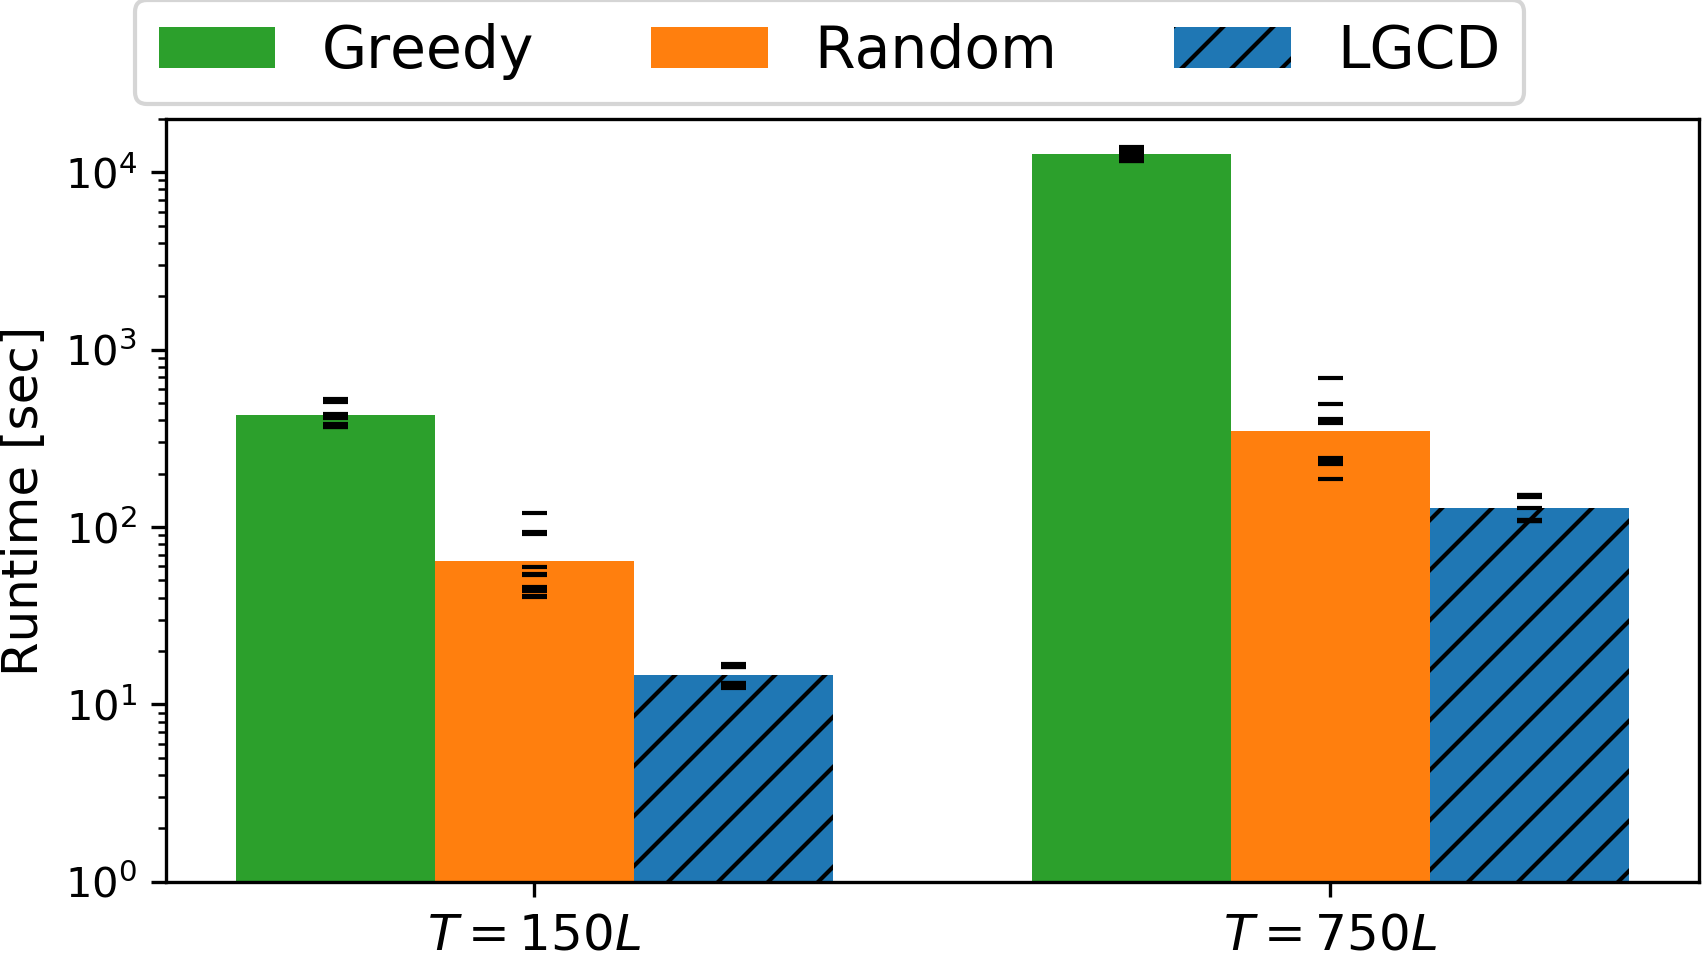
\includegraphics[width=.9\textwidth]{CD_strategies_comparison.png}
% \end{frame}



% \begin{frame}{D-step: solving for the atoms}

% 	We use the projected gradient descent with an Armijo backtracking line-search \cite{Wright1999} for both u-step and v-step for
% 	\begin{equation}
% 		\begin{split}
% 			\min_{\substack{\|u_{k}\|_2 \leq 1\\\|v_{k}\|_2 \leq 1}} E(u_k, v_k) \overset{\Delta}{=} \sum_{n=1}^N\frac{1}{2}\|X^n - \sum_{k=1}^K z^n_k * (u_k^{ }  v_k^\top) \|_{2}^{2} \hspace{6pt}
% 			\enspace .
% 		\end{split}
% 	\end{equation}

% 	One important computation trick is for fast computation of the gradient.
% 	\[
% 	\begin{split}
% 		\nabla_{u_k} E(u_k, v_k) &=  \nabla_{D_k}E(u_k, v_k) v_k ~~ \in \Rset^{P}~,\\
% 		\nabla_{v_k} E(u_k, v_k) &=  u_k^\top \nabla_{D_k} E(u_k, v_k)  ~~ \in \Rset^L~,
% 	\end{split}
% 	\]
% 	Computing $\nabla_{D_k} E(u_k, v_k)$ can be done efficiently
% 	\[
% 	\nabla_{D_{k}} E(u_k, v_k) =  \sum_{n=1}^N (z_k^n)^\Lsh * \left(X^n - \sum_{l=1}^K z^n_l * D_l\right)
% 	=  \Phi_k - \sum_{l=1}^K \Psi_{k, l} *  D_l \enspace ,
% 	\]

% \end{frame}


\begin{frame}{Good scaling in the number of channels $P$}
    Scaling relative to $P$ on somato dataset with $T=134,700$, $K=2$, and $L=128$\\[1em]
    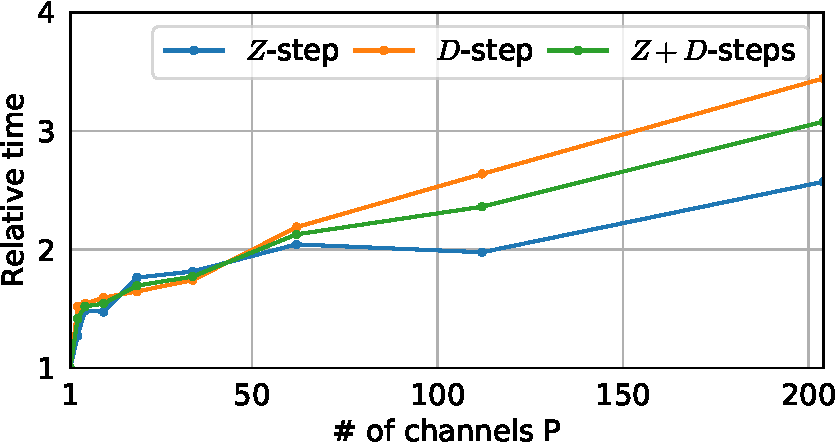
\includegraphics[width=\textwidth]{scaling_channels_reg0_001_mean_rank1_K2_L128.pdf}
\end{frame}

\begin{frame}{Pattern recovery}
Test the pattern recovery capabilities of our method on simulated data,
\[
	X^n = \sum_{k=1}^2 z_k * (u_kv_k^\top) + \mathcal E
\]
where $(u_k, v_k)$ are chosen patterns of rank-1 and the activated coefficient $z^n_k[t]$ are drawn uniformly and their value are uniform in $[0, 1]$.\\[1em]
The noise $\mathcal E$ is generated as a gaussian white noise with variance $\sigma$.\\[1em]

We set $N=100$, $L=64$ and $\tT=640$
\end{frame}

\begin{frame}{Pattern recovery}
Patterns recovered with $P = 1$ and $P=5$. The signals were generated with the two simulated temporal patterns and with  $\sigma = 10^{-3}$. \\[1em]
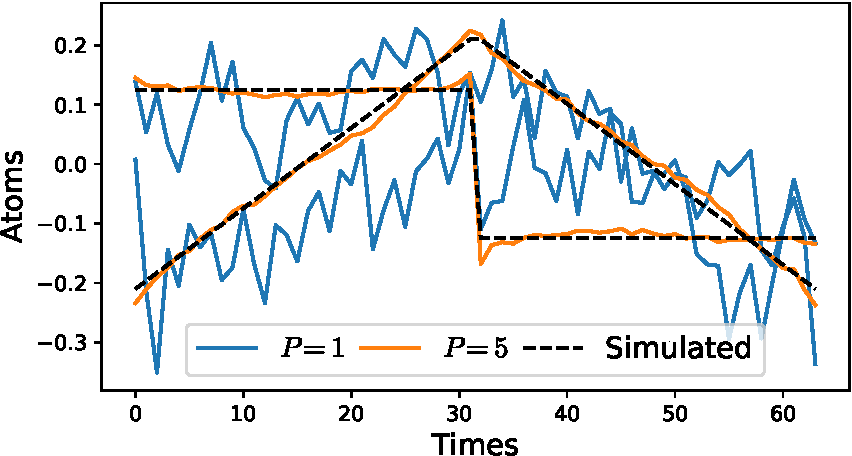
\includegraphics[width=\textwidth]{1D_vs_multi_uv_hat_P5.pdf}
\end{frame}

% \begin{frame}{Pattern recovery}
% Evolution of the recovery loss with $\sigma$ for different values of $P$. Using more channels improves the recovery of the original patterns.\\[1em]
% 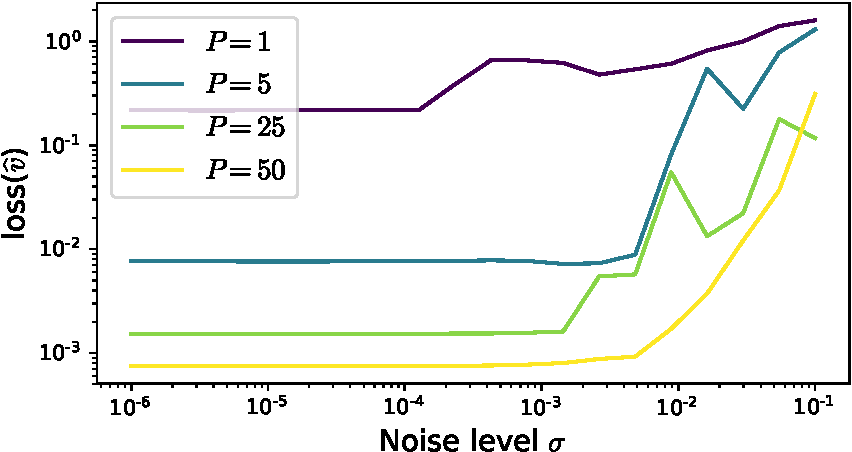
\includegraphics[width=\textwidth]{1D_vs_multi.pdf}
% \end{frame}


\begin{frame}{MNE sample data}
A selection of temporal waveforms of the atoms learned on the MNE sample dataset.\\[1em]
\centering
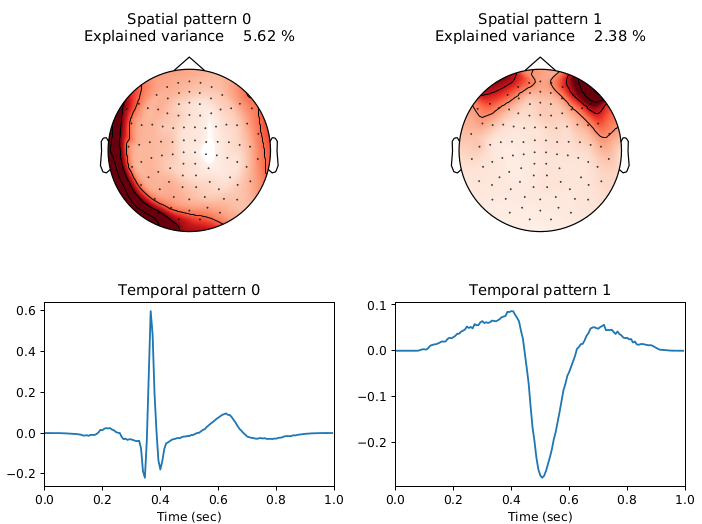
\includegraphics[height=0.7\textheight]{artifacts}
\end{frame}


\frame[t]{
    \frametitle{Learned atoms -- Evoked response}

    \centering
    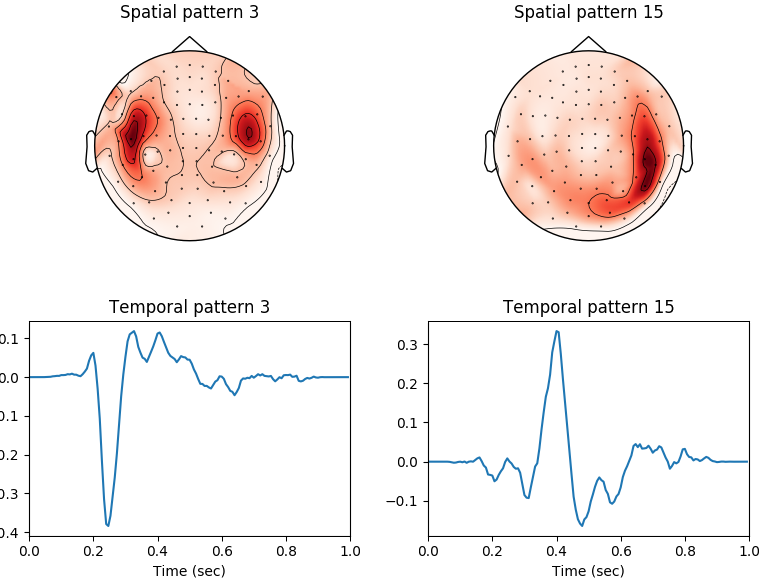
\includegraphics[width=.9\columnwidth]{evoked}
}


\frame[t]{
    \frametitle{Learned atoms -- Induced responses}

    \centering
    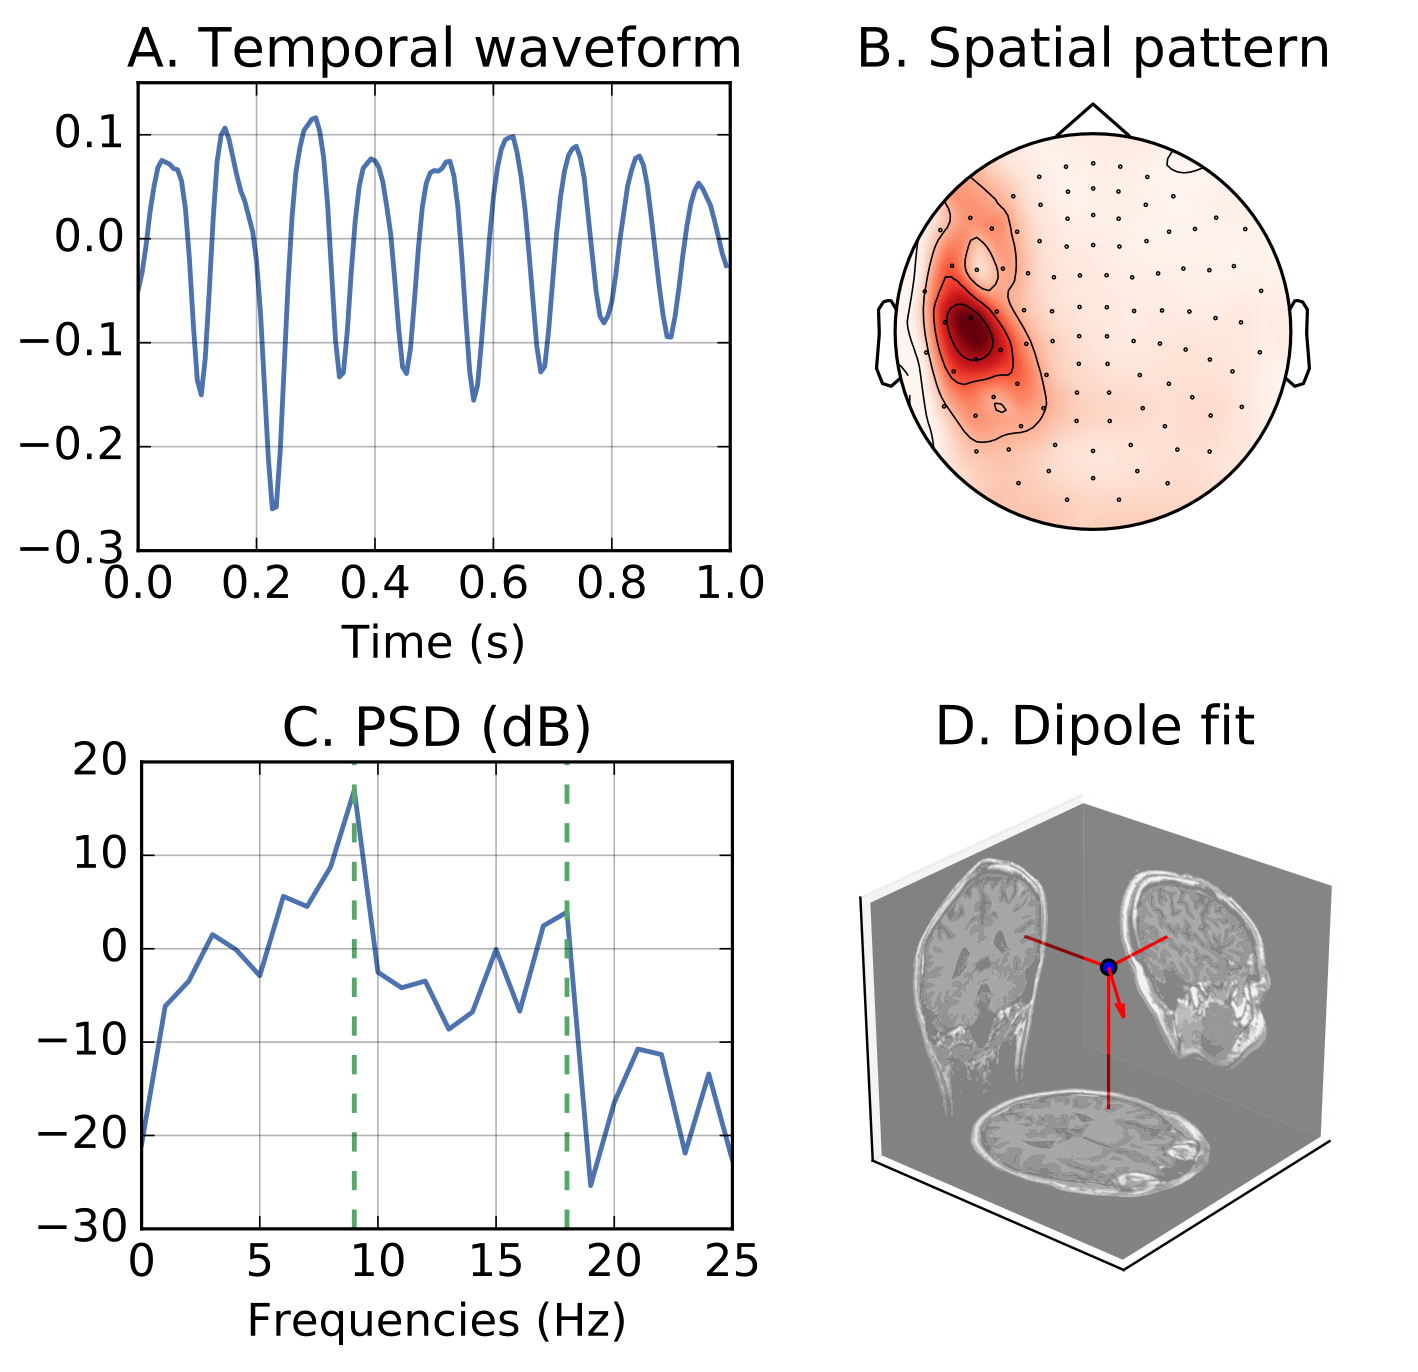
\includegraphics[width=.7\columnwidth]{atom_somato}
}


{\usebackgroundtemplate{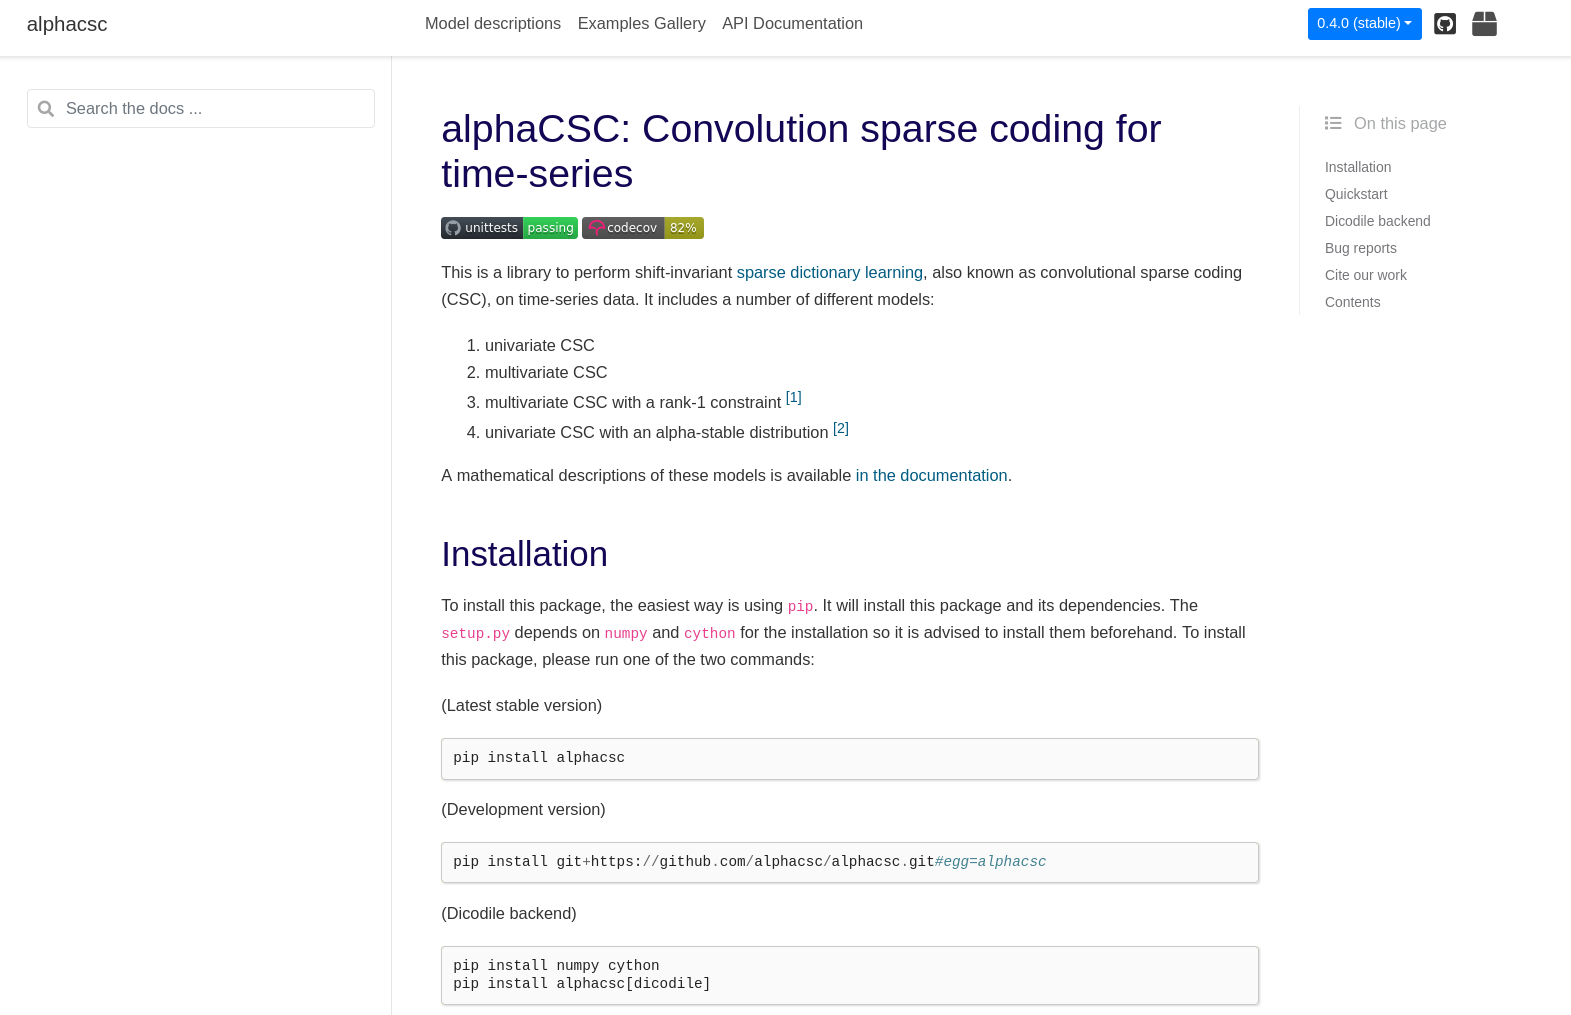
\includegraphics[width=\paperwidth]{alphacsc_04}}%
\frame{
    \begin{columns}
        \column{.5\textwidth}
        \column{.4\textwidth}
        \highlightbox{Python code online:\\
                        https://alphacsc.github.io\\[1em]
                        \texttt{pip install alphacsc}}
        \vskip2em
            \highlightbox{Examples reproduce figures from this talk!}

    \end{columns}
}}


\section{Modeling stimuli induced patterns\\with Point Processes}

\parttitleframe{Allain2022}

\frame{
    \frametitle{Stimuli Induced Patterns}

    \myitem{} Manual pattern identification\\[.5em]
    \myitem{} No quantification of how stimuli influence patterns activation.\\[1em]

    \centering
    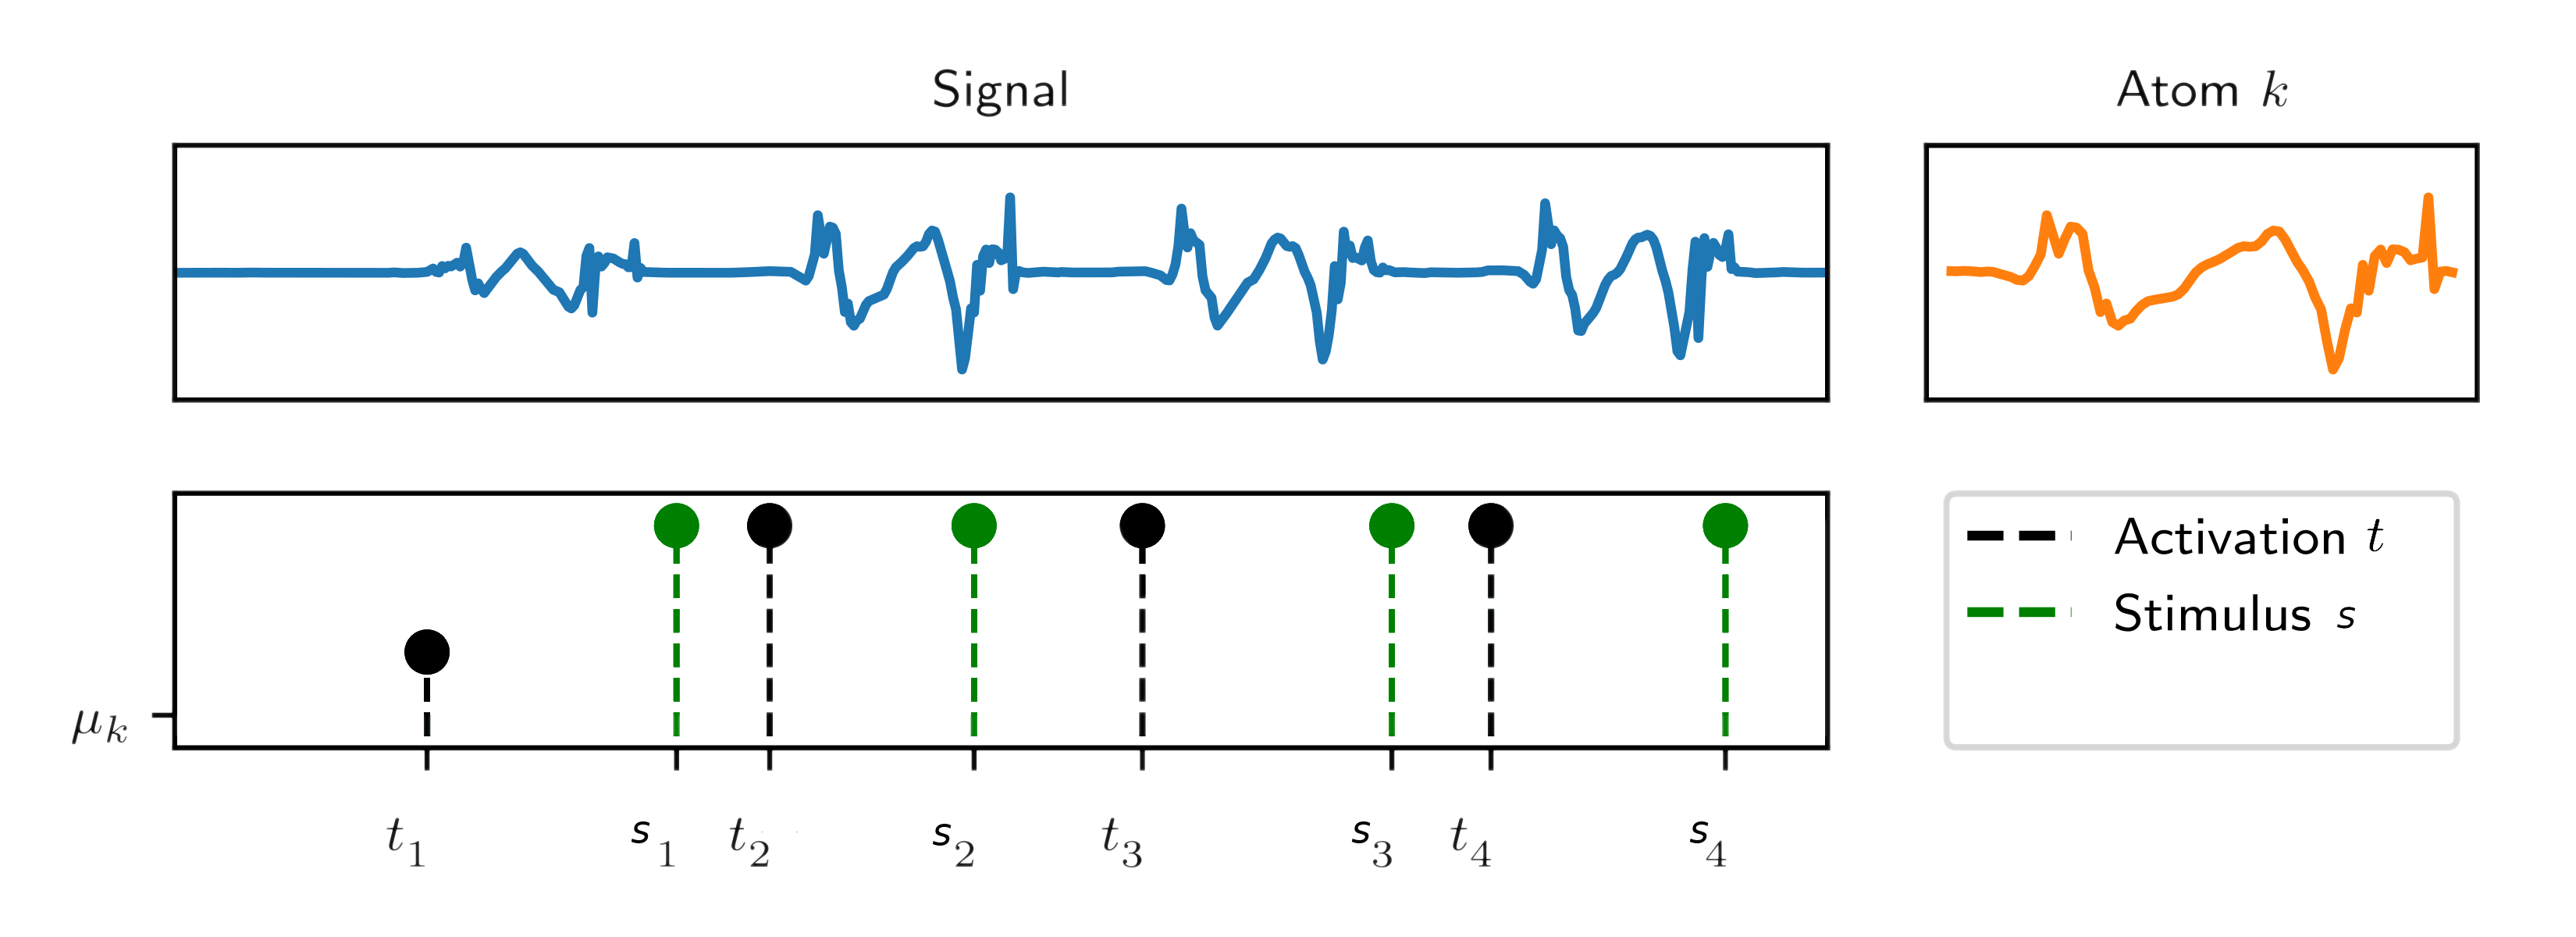
\includegraphics[width=\textwidth]{csc_and_pp_no_intensity.png}\\[1em]


    Activations and stimuli can be seen as \emph{Point Processes}.\\
}

\frame{
    \frametitle{Point Processes \mycite{Daley2003}}

    \begin{itemize}\itemsep.5em
        \item Stochastic model for stream of events
        \item Time of arrival $\{t_k\}$ associated with counting process $N(t)$
        \item Characterized by the intensity:
        \[
            \lambda(t | \mathcal F_t) = \lim_{dt \to 0} \frac{P(N(t+dt) - N(t) = 1 | \mathcal F_t)}{dt}
        \]
    \end{itemize}

    \begin{columns}
        \column{.5\textwidth}
            \centering
            Poisson process with constant probability of arrival
            \[
                \lambda(t) = \mu_0
            \]
        \column{.5\textwidth}
        {\centering
        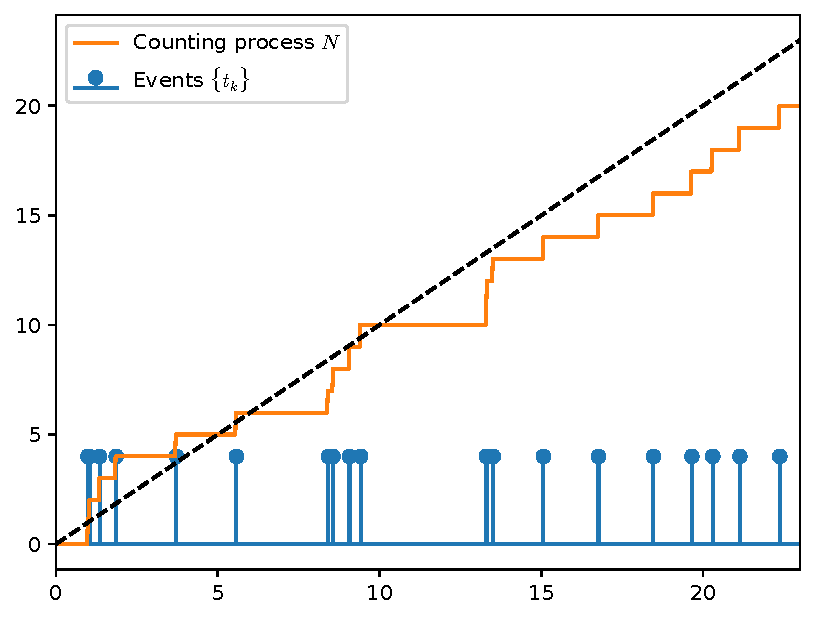
\includegraphics[width=\textwidth]{point_process}\\}
    \end{columns}
}

\frame{
    \frametitle{DriPP -- Driven Point Process}

    {\bf Idea:} Model the probability of activation $\{t_k\}$ depending on the PP from the stimuli $\{s_p\}$.
    \[
        \lambda(t | \mathcal F_t) = \lambda(t | \{s_p; s_p < t\}) = \mu_0 + \sum_{s_p < t} \kappa(t - s_p)
    \]

    \centering
    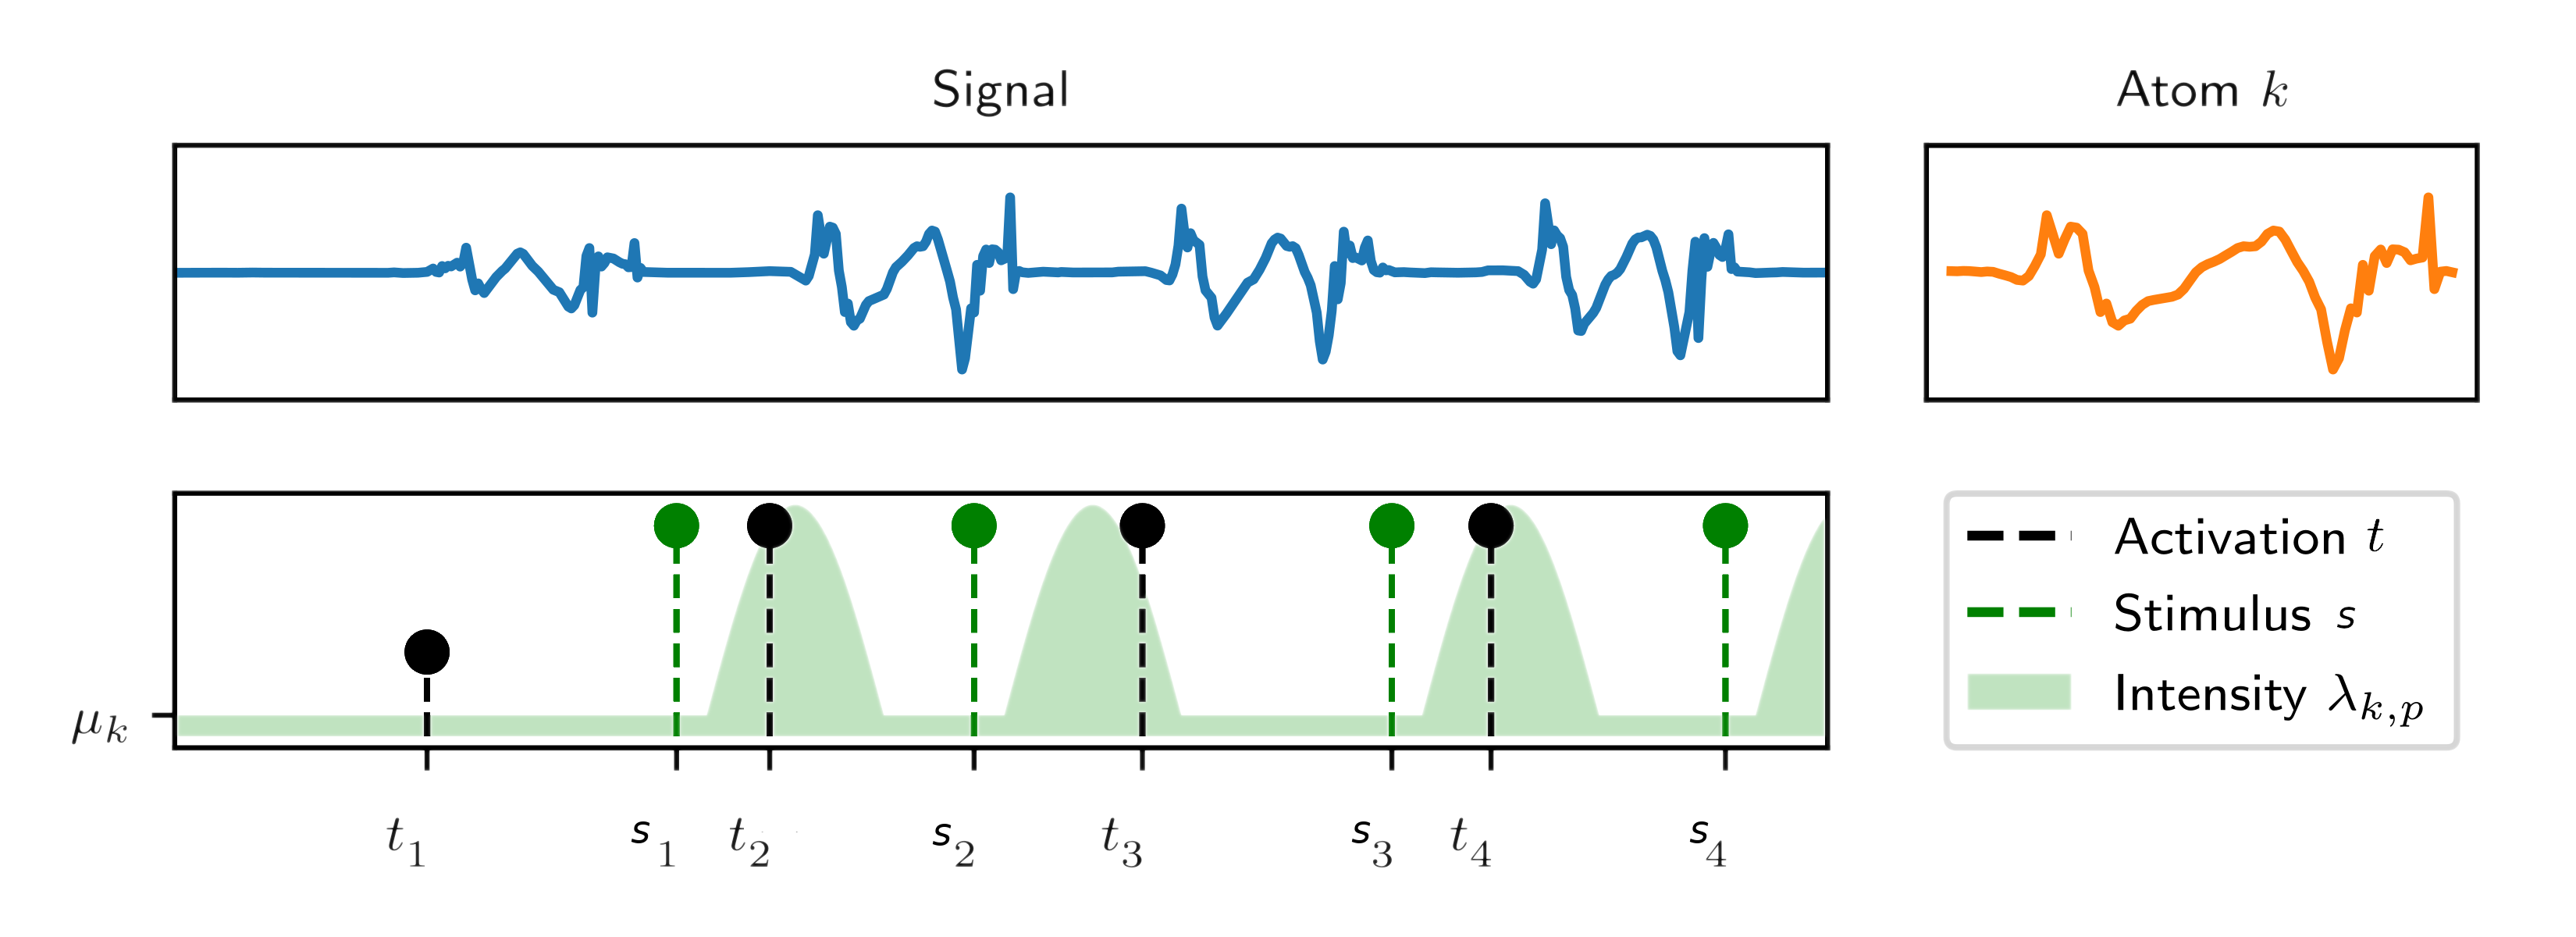
\includegraphics[width=\textwidth]{csc_and_pp.png}\\[1em]


    % Activations and stimuli can be seen as \emph{Point Processes}.\\
}

\frame{
    \frametitle{Modeling latency}

    Chosing a model for stimuli based modeling:
    \[
        \lambda(t | \mathcal F_t) = \mu_0 + \sum_{s_p < t} \alpha\kappa(t - s_p)
    \]

    \begin{columns}

        \column{.5\textwidth}
        \begin{itemize}
            \item $\mu_0 \ge 0$: spontaneous activity.
            \item $\alpha \ge 0$: allow for stimuli to have no effect.
            \item $\kappa(\tau)$: pdf of a truncated Gaussian $\mathcal N(m, \sigma^2)$ to model latency.
        \end{itemize}
        \column{.5\textwidth}
        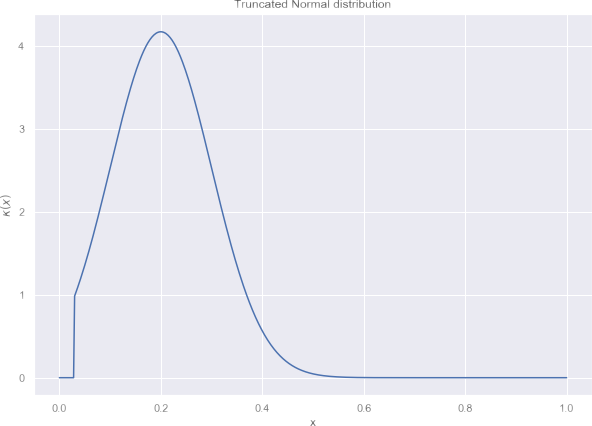
\includegraphics[width=\textwidth]{trunc_norm_distribution}
    \end{columns}
}

\frame{
    \frametitle{Parameters estimation}

    The negative log-likelihood of the model can be computed using the intensity $\lambda$:
    \begin{align*}
        \mathcal L(\{t_k\}; \Theta) &= \int_0^T \lambda(t ) dt -\sum_{t_k} \log \lambda(t_k)\\
        & = \mu_0 T + \alpha |\{t_k\}| - \sum_{t_k} \log(\mu_0\sum_{s_p < t_k} \alpha\kappa(t_k - s_p))
    \end{align*}
    with $\Theta = (\mu_0, \alpha, m, \sigma^2)$\\[1em]

    \strongpoint{Parameter estimation with an EM algorithm.}
}


% \frame{
%     \frametitle{Parameters recovery}

%     Events simulated with the Truncated Gaussian model:
%     {\centering
%     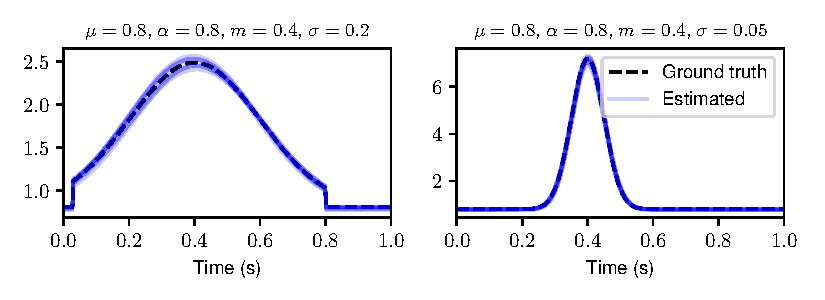
\includegraphics[width=.8\textwidth]{kernel_recovery}\\
%     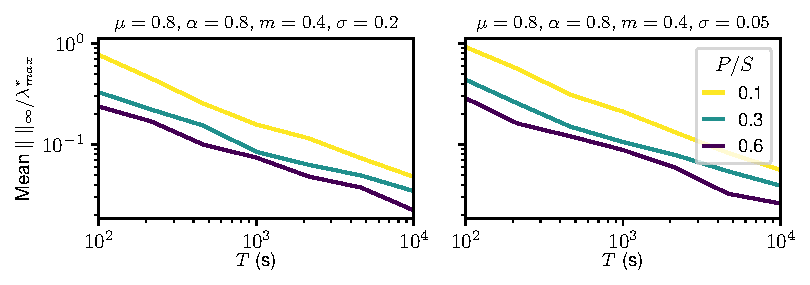
\includegraphics[width=.8\textwidth]{mean_recovery}\\
%     }
% }


\frame{
    \frametitle{Results for artifacts and evoked atoms - samples}

    {\centering
    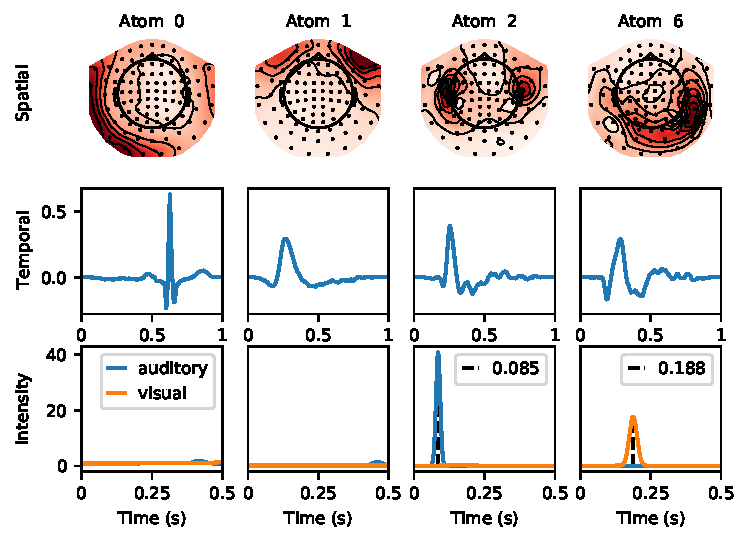
\includegraphics[width=.8\textwidth]{atom_evoked_sample}\\
    }
}


\frame{
    \frametitle{Results for artifacts and evoked atoms - somato}

    {\centering
    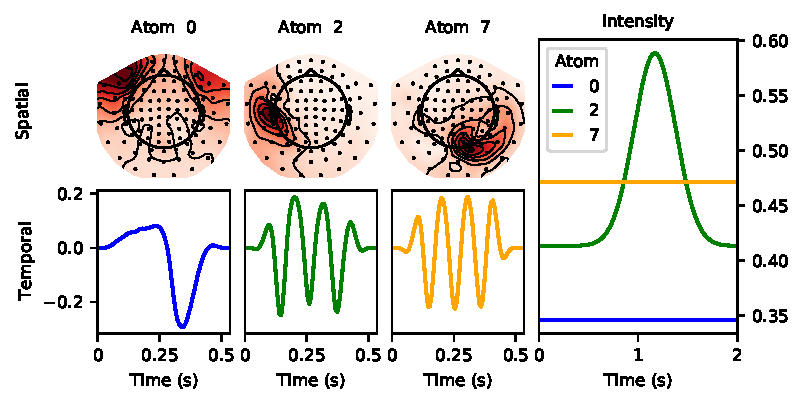
\includegraphics[width=.8\textwidth]{atom_induced_somato}\\
    }
}


\frame{
    \frametitle{Results for artifacts and evoked atoms - somato}

    {\centering
    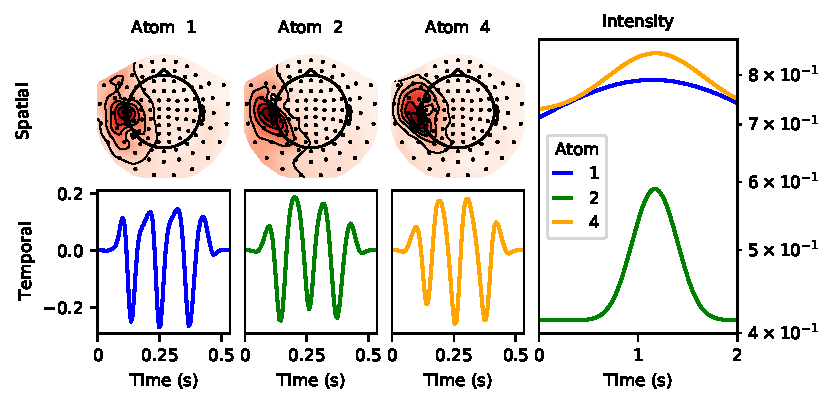
\includegraphics[width=.8\textwidth]{atom_induced_somato_wave}\\
    }
}

\frame{
    \frametitle{Conclusion}

    \begin{itemize}\itemsep1em
    \item CDL can learn recurring patterns in multivariate signals.
    \item Converts the signal into a stream of events.
    \item PP framework can model the activation distribution.
    \end{itemize}

    \vskip2em
    {\bf Limitations and on-going work:}\\[1.5em]
    \begin{itemize}\itemsep1em
        \item Not easy to apply to population level.
        \item DriPP does not model inhibition.
        \item CDL and PP are separated.
    \end{itemize}
}

\section{Benchopt}
\parttitleframe{Moreau2022}



%%%%%%%%%%%%%%%%%%%%%%%%%%%%%%%%%%%%%%%%%%%%%%%%%%%%%%%%%%%%%%%%%%%%%%%%%%%%%%%
\begin{frame}[fragile]{\texttt{benchopt}}

Doing a  benchmark for the $\ell_2$ regularized logistic regression with multiple solvers and datasets is now easy as calling:\\[1em]

\begin{lstlisting}[language=bash]
git clone https://github.com/benchopt/benchmark_logreg_l2
benchopt run ./benchmark_logreg_l2
\end{lstlisting}

\vskip.5em
{   \centering
    \includegraphics[width=.55\textwidth]{plot_run_benchmark.png}\\
}
% \hskip3ex
% \includegraphics[width=.45\textwidth]{logreg_l2_1}

\end{frame}
%%%%%%%%%%%%%%%%%%%%%%%%%%%%%%%%%%%%%%%%%%%%%%%%%%%%%%%%%%%%%%%%%%%%%%%%%%%%%%%


%%%%%%%%%%%%%%%%%%%%%%%%%%%%%%%%%%%%%%%%%%%%%%%%%%%%%%%%%%%%%%%%%%%%%%%%%%%%%%%
\begin{frame}{Benchmark: principle}

A benchmark is a directory with:\\
\begin{itemize}
    \item An \lstinline+objective.py+ file with an \lstinline+Objective+
    \item A directory \lstinline+solvers+ with one file per \lstinline+Solver+
    \item A directory \lstinline+datasets+ with \lstinline+Dataset+ generators/fetchers
\end{itemize}
\vskip1em

\includegraphics[width=.9\textwidth,trim={0 0 0 2.8em},clip]{benchopt_structure}

\vskip1em
The \lstinline+benchopt+ client runs a cross product and generates a csv file + convergence plots like above.
\end{frame}
%%%%%%%%%%%%%%%%%%%%%%%%%%%%%%%%%%%%%%%%%%%%%%%%%%%%%%%%%%%%%%%%%%%%%%%%%%%%%%%

%%%%%%%%%%%%%%%%%%%%%%%%%%%%%%%%%%%%%%%%%%%%%%%%%%%%%%%%%%%%%%%%%%%%%%%%%%%%%%%
\frame{
    \frametitle{Benchopt: principle}

    \includegraphics[width=\textwidth]{benchopt_schema_objectives_with_logos}

    \strongpoint{Each object can be parametrized so multiple scenario can be tested.}
}


%%%%%%%%%%%%%%%%%%%%%%%%%%%%%%%%%%%%%%%%%%%%%%%%%%%%%%%%%%%%%%%%%%%%%%%%%%%%%%%
\begin{frame}{\texttt{benchopt: Making tedious tasks easy}}

    {\bf Automatizing tasks:}\\[1.2em]
    \begin{itemize}\itemsep.7em
        \item Automatic installation of competitors solvers.
        \item Parametrized datasets, objectives and solvers and run on cross products.
        \item Make sure to quantify the variance.
        \item Automatic caching.
        \item Interactive visualization of the results
        \item Automatic parallelization, run on SLURM,
        \item ...?
    \end{itemize}
\end{frame}
%%%%%%%%%%%%%%%%%%%%%%%%%%%%%%%%%%%%%%%%%%%%%%%%%%%%%%%%%%%%%%%%%%%%%%%%%%%%%%%


\frame{
    \vskip2em
    {\centering
        \usebeamercolor[fg]{title}
        \usebeamerfont{title}
        \Huge \bf Thanks for your attention!\\[2em]}

    Code available online:\\[1em]

    \includegraphics[height=.8em]{github}~\textbf{alphacsc} :  alphacsc.github.io\\[1em]
    \includegraphics[height=.8em]{github}~\textbf{DriPP} : github.com/CedricAllain/dripp\\[1em]
    \includegraphics[height=.8em]{github}~\textbf{benchopt} : benchopt.github.io\\[2em]

    Slides are on my web page:\\[1em]
    \hskip5em\includegraphics[height=.8em]{website} tommoral.github.io
    \hskip4em \includegraphics[height=.8em]{twitter} @tomamoral

}



\appendix


\begin{frame}{Fast optimization}
Comparison with univariate methods on somato dataset with $T=134,700$, $K=8$ and $L=128$\\[1em]
\includegraphics[width=\textwidth]{all_last_0001_T_13470_P1_K8_L128}
\end{frame}

\begin{frame}{Fast optimization}
Comparison with multivariate methods on somato dataset with $T=134,700$, $K=8$, $P=5$ and $L=128$\\[1em]
\includegraphics[width=\textwidth]{all_last_0001_T_13470_P5_K8_L128}
\end{frame}


\end{document}
